\documentclass[aspectratio=169,10pt]{beamer}

% Packages
\usepackage[utf8]{inputenc}
\usepackage[T1]{fontenc}
\usepackage{graphicx}
\usepackage{booktabs}
\usepackage{array}
\usepackage{xcolor}
\usepackage{tikz}
\usepackage{helvet}
\renewcommand{\familydefault}{\sfdefault}

% University of Bristol Color Palette
\definecolor{BristolRed}{RGB}{176, 28, 46}       % #B01C2E
\definecolor{BristolDarkRed}{RGB}{140, 20, 36}   % #8C1424
\definecolor{BristolNavy}{RGB}{12, 35, 64}       % #0C2340
\definecolor{BristolCharcoal}{RGB}{30, 41, 59}   % #1E293B
\definecolor{BristolSlate}{RGB}{100, 116, 139}   % #64748B
\definecolor{BristolBg}{RGB}{248, 250, 252}      % #F8FAFC
\definecolor{BristolCard}{RGB}{255, 255, 255}
\definecolor{BristolBorder}{RGB}{226, 232, 240}
\definecolor{BristolAccent}{RGB}{217, 83, 30}

% Beamer Theme Customization
\setbeamercolor{background canvas}{bg=BristolBg}
\setbeamercolor{normal text}{fg=BristolCharcoal}
\setbeamercolor{frametitle}{fg=BristolNavy,bg=white}
\setbeamercolor{structure}{fg=BristolRed}
\setbeamercolor{item}{fg=BristolRed}
\setbeamercolor{block title}{fg=white,bg=BristolRed}
\setbeamercolor{block body}{fg=BristolCharcoal,bg=white}

\setbeamertemplate{navigation symbols}{}

% Header and Footer
\setbeamertemplate{headline}{
  \begin{tikzpicture}[remember picture,overlay]
    \fill[BristolRed] (current page.north west) rectangle ([yshift=-2pt]current page.north east);
  \end{tikzpicture}
}

\setbeamertemplate{footline}{
  \leavevmode%
  \hbox{%
    \begin{beamercolorbox}[wd=\paperwidth,ht=2.5ex,dp=1.125ex,leftskip=1cm,rightskip=1cm]{author in head/foot}%
      \textcolor{BristolSlate}{\scriptsize University of Bristol \quad\textbar\quad MSc Data Science Final Group Dissertation \quad\textbar\quad 16 September 2026 \hfill \insertframenumber{} / \inserttotalframenumber}
    \end{beamercolorbox}%
  }%
  \vskip0pt%
}

% Custom Frame Title
\setbeamertemplate{frametitle}{
  \vspace{0.3cm}
  \begin{beamercolorbox}[wd=\textwidth,ht=1.0cm,dp=0.2cm]{frametitle}
    \begin{minipage}[c]{0.82\textwidth}
      {\tiny \textbf{\textcolor{BristolRed}{\insertsectionhead\ \textbar\ Slide \insertframenumber}}}\\[1pt]
      {\large \textbf{\textcolor{BristolNavy}{\insertframetitle}}}
    \end{minipage}
    \begin{minipage}[c]{0.16\textwidth}
      \flushright
      
\includegraphics[width=2.2cm,keepaspectratio]{logo_uob_color.png}
    \end{minipage}
  \end{beamercolorbox}
  \vspace{-0.2cm}
}

\title[Edge-Deployable Rock Detection]{Edge-Deployable Rock Detection and Burial-Status Classification}
\subtitle{Real-Time Embedded Computer Vision for Precision Agriculture on Raspberry Pi 5}
\author{1. Tanishk Nanasaheb Shinde \and 2. Megh Kashilkar \and 3. Sanskar Gade \and 4. Jitendra Suwalka}
\institute{University of Bristol \and Dalhousie University / McCain Foods}
\date{16th September, 2026}

\begin{document}

% -------------------------------------------------------------
% SLIDE 1: Title Slide (WHITE & RED UNIVERSITY COLOURS)
% -------------------------------------------------------------
{
\setbeamertemplate{headline}{}
\setbeamertemplate{footline}{}
\begin{frame}[plain]
  \begin{tikzpicture}[remember picture,overlay]
    \fill[BristolBg] (current page.north west) rectangle (current page.south east);
    \fill[BristolRed] (current page.north west) rectangle ([yshift=-4pt]current page.north east);
  \end{tikzpicture}
  
  \vspace{-0.3cm}
  \begin{columns}[c]
    \begin{column}{0.60\textwidth}
      
\includegraphics[height=1.05cm,keepaspectratio]{logo_uob_color.png}
    \end{column}
    \begin{column}{0.38\textwidth}
      \flushright
      {\scriptsize \textbf{\textcolor{BristolSlate}{MSc Data Science Dissertation}}\\[1pt]
      {\tiny \textcolor{BristolSlate}{Final Group Project Presentation}}}
    \end{column}
  \end{columns}
  
  \vspace{0.3cm}
  \begin{beamercolorbox}[wd=\textwidth,sep=0pt]{title}
    {\Large \textbf{\textcolor{BristolNavy}{Edge-Deployable Rock Detection\\[2pt]\& Burial-Status Classification}}}\\[4pt]
    {\footnotesize \textbf{\textcolor{BristolRed}{Real-Time Embedded Computer Vision for Precision Agriculture on Raspberry Pi 5}}}
  \end{beamercolorbox}
  
  \vspace{0.35cm}
  
\begin{tikzpicture}
    \node[draw=BristolBorder, line width=0.8pt, fill=white, rounded corners=4pt, inner sep=8pt, text width=0.94\textwidth] {
      {\footnotesize \textbf{\textcolor{BristolNavy}{Project Team:}} \textbf{\textcolor{BristolCharcoal}{1. Tanishk Nanasaheb Shinde \quad 2. Megh Kashilkar \quad 3. Sanskar Sanju Gade \quad 4. Jitendra Suwalka}}}\\[4pt]
      {\scriptsize \textbf{\textcolor{BristolNavy}{Academic Supervisor:}} \textcolor{BristolCharcoal}{Dr. Felipe Campelo (University of Bristol)}}\\[2pt]
      {\scriptsize \textbf{\textcolor{BristolNavy}{External Supervisors:}} \textcolor{BristolCharcoal}{Dr. Ahmad Al-Mallahi \& Jason McLaren (Dalhousie University / McCain Foods)}}\\[4pt]
      {\tiny \textcolor{BristolSlate}{University of Bristol \quad\textbar\quad Faculty of Engineering \quad\textbar\quad Department of Engineering Mathematics \quad\textbar\quad 16 September 2026}}
    };
  \end{tikzpicture}
\end{frame}
}

% -------------------------------------------------------------
% SLIDE 2: Agricultural Problem
% -------------------------------------------------------------
\section{Context \& Motivation}
\begin{frame}{Rocks Cause Severe Operational \& Equipment Costs in Potato Farming}
\begin{columns}[T]
  \begin{column}{0.48\textwidth}
    \begin{block}{\small Operational Challenge \& Need}
      \small
      \begin{itemize}
        \item Field rocks obstruct tillage, damage mechanical harvester blades, and puncture sorting equipment.
        \item Harvesting downtime and manual rock picking represent significant commercial bottlenecks.
        \item Removing rocks requires knowing both \textbf{location} and \textbf{burial status} (completely exposed vs half-buried) to calibrate actuation force.
      \end{itemize}
    \end{block}
  \end{column}
  \begin{column}{0.48\textwidth}
    \begin{block}{\small Industry Collaboration Objectives}
      \small
      \begin{itemize}
        \item \textbf{Partner:} McCain Foods \& Dalhousie University.
        \item \textbf{Goal:} Real-time vision deployed directly on field tractors.
        \item \textbf{Constraint:} Rural fields lack continuous cloud connectivity, demanding \textbf{fully offline edge inference}.
        \item \textbf{Target:} Low-cost embedded compute (Raspberry Pi 5).
      \end{itemize}
    \end{block}
  \end{column}
\end{columns}
\end{frame}

% -------------------------------------------------------------
% SLIDE 3: Edge-Deployment Challenge
% -------------------------------------------------------------
\begin{frame}{High Model Accuracy Does Not Guarantee Real-Time Edge Feasibility}
\begin{columns}[T]
  \begin{column}{0.48\textwidth}
    \begin{block}{\small The Academic vs Edge Deployment Gap}
      \small
      \begin{itemize}
        \item Standard research relies on GPU servers with FP32 precision.
        \item Tractor operations at 5--10~km/h require \textbf{$\ge$ 15--20 FPS} for real-time hydraulic rock picker guidance.
        \item Baseline PyTorch on Raspberry Pi 5 runs at only \textbf{2.52 FPS (397 ms latency)} --- unusable for live control.
        \item Quantisation (FP16/INT8) and embedded runtimes (TFLite/NCNN) are mandatory.
      \end{itemize}
    \end{block}
  \end{column}
  \begin{column}{0.48\textwidth}
    \begin{block}{\small Edge Physical Constraints}
      \small
      \begin{itemize}
        \item \textbf{Compute:} Quad-core ARM Cortex-A76 without discrete GPU.
        \item \textbf{Power \& Heat:} Enclosed tractor cabs with passive cooling risk thermal CPU throttling.
        \item \textbf{Memory:} Must operate reliably within limited RAM without paging.
        \item \textbf{Stability:} 100\% crash-free continuous execution required.
      \end{itemize}
    \end{block}
  \end{column}
\end{columns}
\end{frame}

% -------------------------------------------------------------
% SLIDE 4: Research Question & Hypotheses
% -------------------------------------------------------------
\begin{frame}{Core Research Question \& Empirical Hypotheses}
\begin{columns}[T]
  \begin{column}{0.48\textwidth}
    \begin{block}{\small Central Research Question}
      \small
      \textit{``How effectively can lightweight YOLO models be optimised, quantised, and deployed for real-time rock detection and burial-status classification on a low-cost edge device (Raspberry Pi 5)?''}
      \vspace{4pt}
      \begin{itemize}
        \item \textbf{Q1:} What is the best architecture for exposed vs half-buried rocks?
        \item \textbf{Q2:} What are the empirical trade-offs between precision, speed, memory, and stability?
      \end{itemize}
    \end{block}
  \end{column}
  \begin{column}{0.48\textwidth}
    \begin{block}{\small Guiding Hypotheses}
      \small
      \begin{itemize}
        \item \textbf{H1 (Speedup):} Quantised runtimes (TFLite INT8 / NCNN) will yield $\ge 5\times$ latency reduction over PyTorch baseline.
        \item \textbf{H2 (Accuracy Cost):} INT8 quantisation will incur a measurable localisation penalty ($\text{mAP} drop < 5\%$).
        \item \textbf{H3 (Operational Divergence):} Runtimes will show significant divergence in CPU load, thermals, and endurance stability.
      \end{itemize}
    \end{block}
  \end{column}
\end{columns}
\end{frame}

% -------------------------------------------------------------
% SLIDE 5: Methodology Overview
% -------------------------------------------------------------
\section{Methodology Overview}
\begin{frame}{Rigorous Five-Stage End-to-End Project Architecture}
\begin{columns}[T]
  \begin{column}{0.48\textwidth}
    \begin{block}{\footnotesize 5-Stage Execution Pipeline}
      \footnotesize
      \begin{enumerate}\setlength{\itemsep}{1pt}
        \item \textbf{Leakage-Free Splitting:} 313 Train / 45 Val / 90 Test images partitioned \textit{before} augmentation.
        \item \textbf{Controlled Augmentation:} 6 safe photometric transforms expanding training to 2,191 images (3,563 rocks).
        \item \textbf{Controlled Detector Selection:} YOLOv8n, YOLO11n, YOLO11s trained identically; selection via validation mAP50--95.
        \item \textbf{Six-Format Edge Export:} PyTorch, TorchScript, ONNX, TFLite (FP32/INT8), NCNN (FP32/FP16).
        \item \textbf{Pi 5 Benchmark:} Fixed 90-image test + 10-pass endurance run measuring speed, quality, RAM, and thermals.
      \end{enumerate}
    \end{block}
  \end{column}
  \begin{column}{0.48\textwidth}
    \begin{block}{\footnotesize Strict Experimental Controls}
      \footnotesize
      \begin{itemize}\setlength{\itemsep}{2pt}
        \item \textbf{Zero Test Leakage:} Test partition remained untouched throughout development.
        \item \textbf{Constant Neural Weights:} Frozen weights exported across all six runtimes.
        \item \textbf{Standard Letterboxing:} $640\times640$ with symmetric fill (value 114).
        \item \textbf{Systematic Telemetry:} CPU, RAM, and thermals tracked at 10~ms intervals.
      \end{itemize}
    \end{block}
  \end{column}
\end{columns}
\end{frame}

% -------------------------------------------------------------
% SLIDE 6: Dataset Composition
% -------------------------------------------------------------
\section{Dataset Preparation}
\begin{frame}{Original Field Dataset: 448 Images \& 706 Annotated Rocks}
\begin{columns}[T]
  \begin{column}{0.48\textwidth}
    \begin{block}{\small Class Balance \& Distribution}
      \small
      \begin{itemize}
        \item \textbf{448 field images} collected from real potato cultivation plots.
        \item \textbf{706 ground-truth rock annotations}:
        \begin{itemize}
          \item \textbf{Completely Exposed:} 362 objects (51.3\%) --- clear boundaries, high surface contrast.
          \item \textbf{Half-Buried:} 344 objects (48.7\%) --- partial soil occlusion, irregular silhouettes.
        \end{itemize}
        \item Closely balanced (51.3\% vs 48.7\%) totals allow performance differences to be interpreted as visual difficulty rather than class imbalance.
      \end{itemize}
    \end{block}
  \end{column}
  \begin{column}{0.48\textwidth}
    \centering
    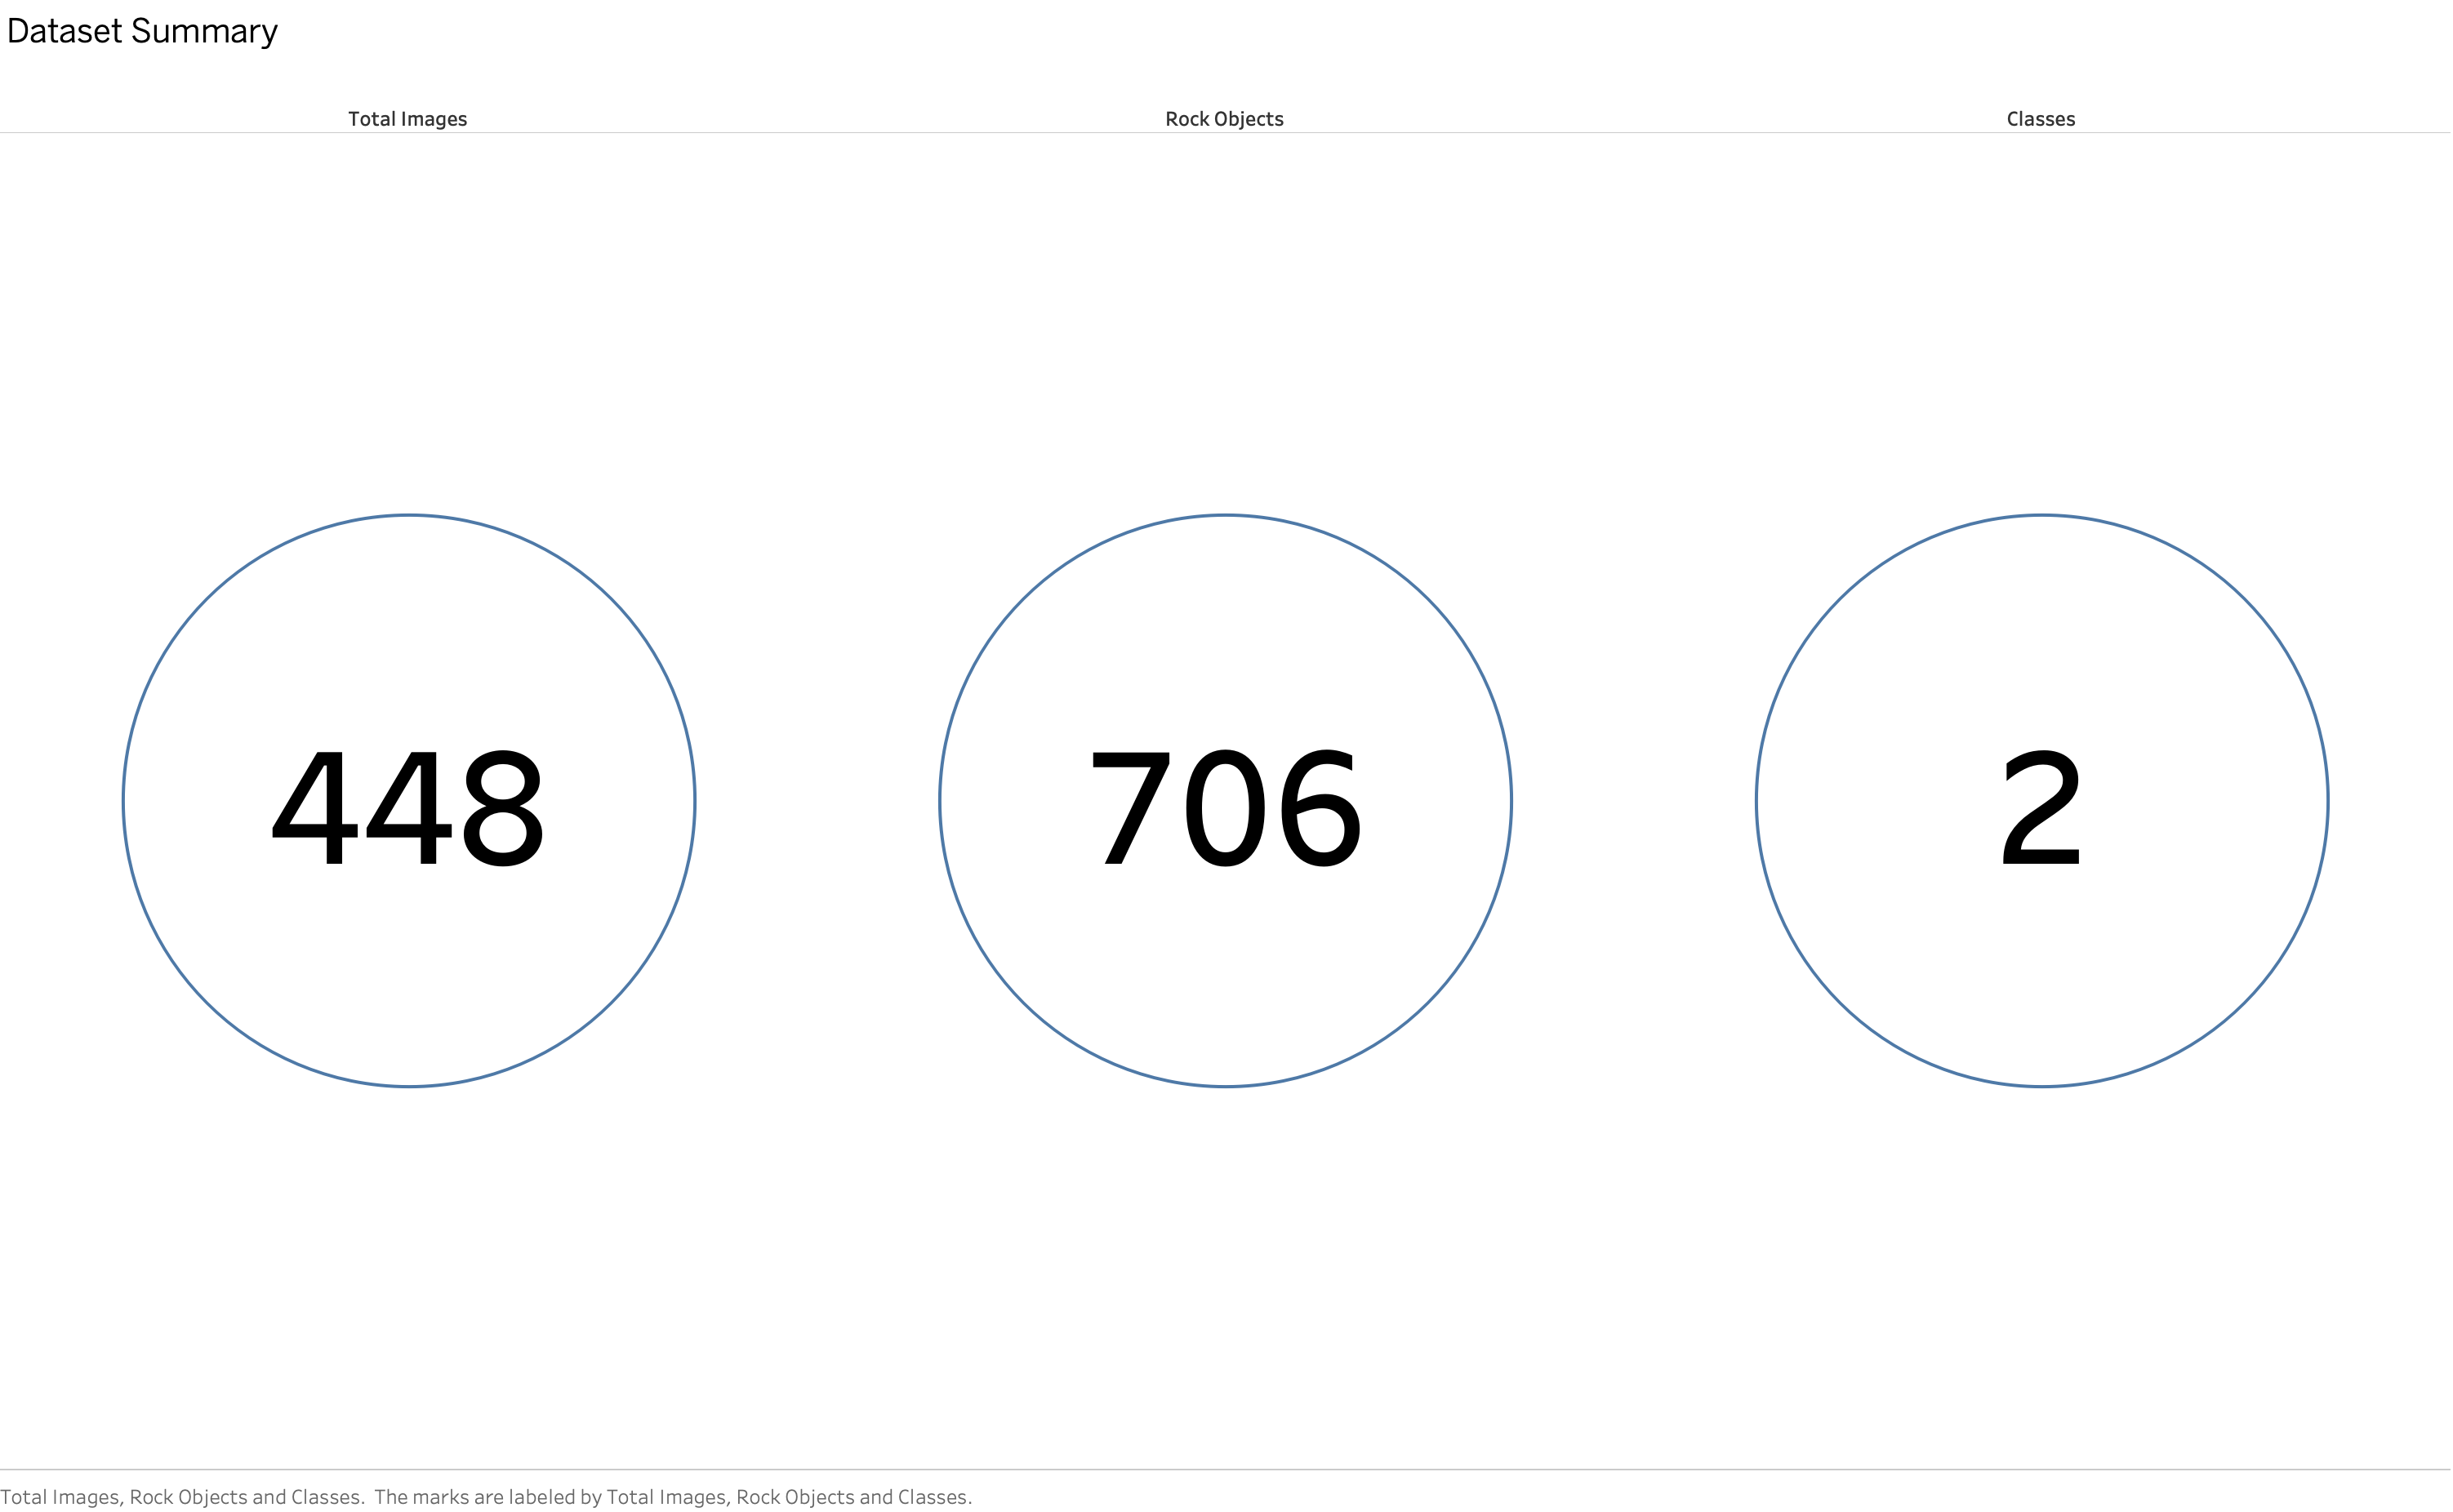
\includegraphics[width=\textwidth,height=4.2cm,keepaspectratio]{figures/figure_04.png}\\[2pt]
    {\tiny Figure 3.4: Dataset summary showing 448 images and 706 annotated rocks.}
  \end{column}
\end{columns}
\end{frame}

% -------------------------------------------------------------
% SLIDE 7: Splitting First
% -------------------------------------------------------------
\begin{frame}{Pre-Augmentation Splitting Prevents Data Leakage}
\begin{columns}[T]
  \begin{column}{0.48\textwidth}
    \begin{block}{\small Partitioning Strategy}
      \small
      \begin{itemize}
        \item Split performed \textbf{prior to augmentation} to ensure zero augmented copies leaked into validation or test sets.
        \item \textbf{Training (313 images):} 259 exposed, 250 half-buried rocks (69.9\%).
        \item \textbf{Validation (45 images):} 34 exposed, 28 half-buried rocks (10.0\%).
        \item \textbf{Test (90 images):} 69 exposed, 66 half-buried rocks (20.1\%).
        \item Preserves absolute independence for edge benchmarking.
      \end{itemize}
    \end{block}
  \end{column}
  \begin{column}{0.48\textwidth}
    \centering
    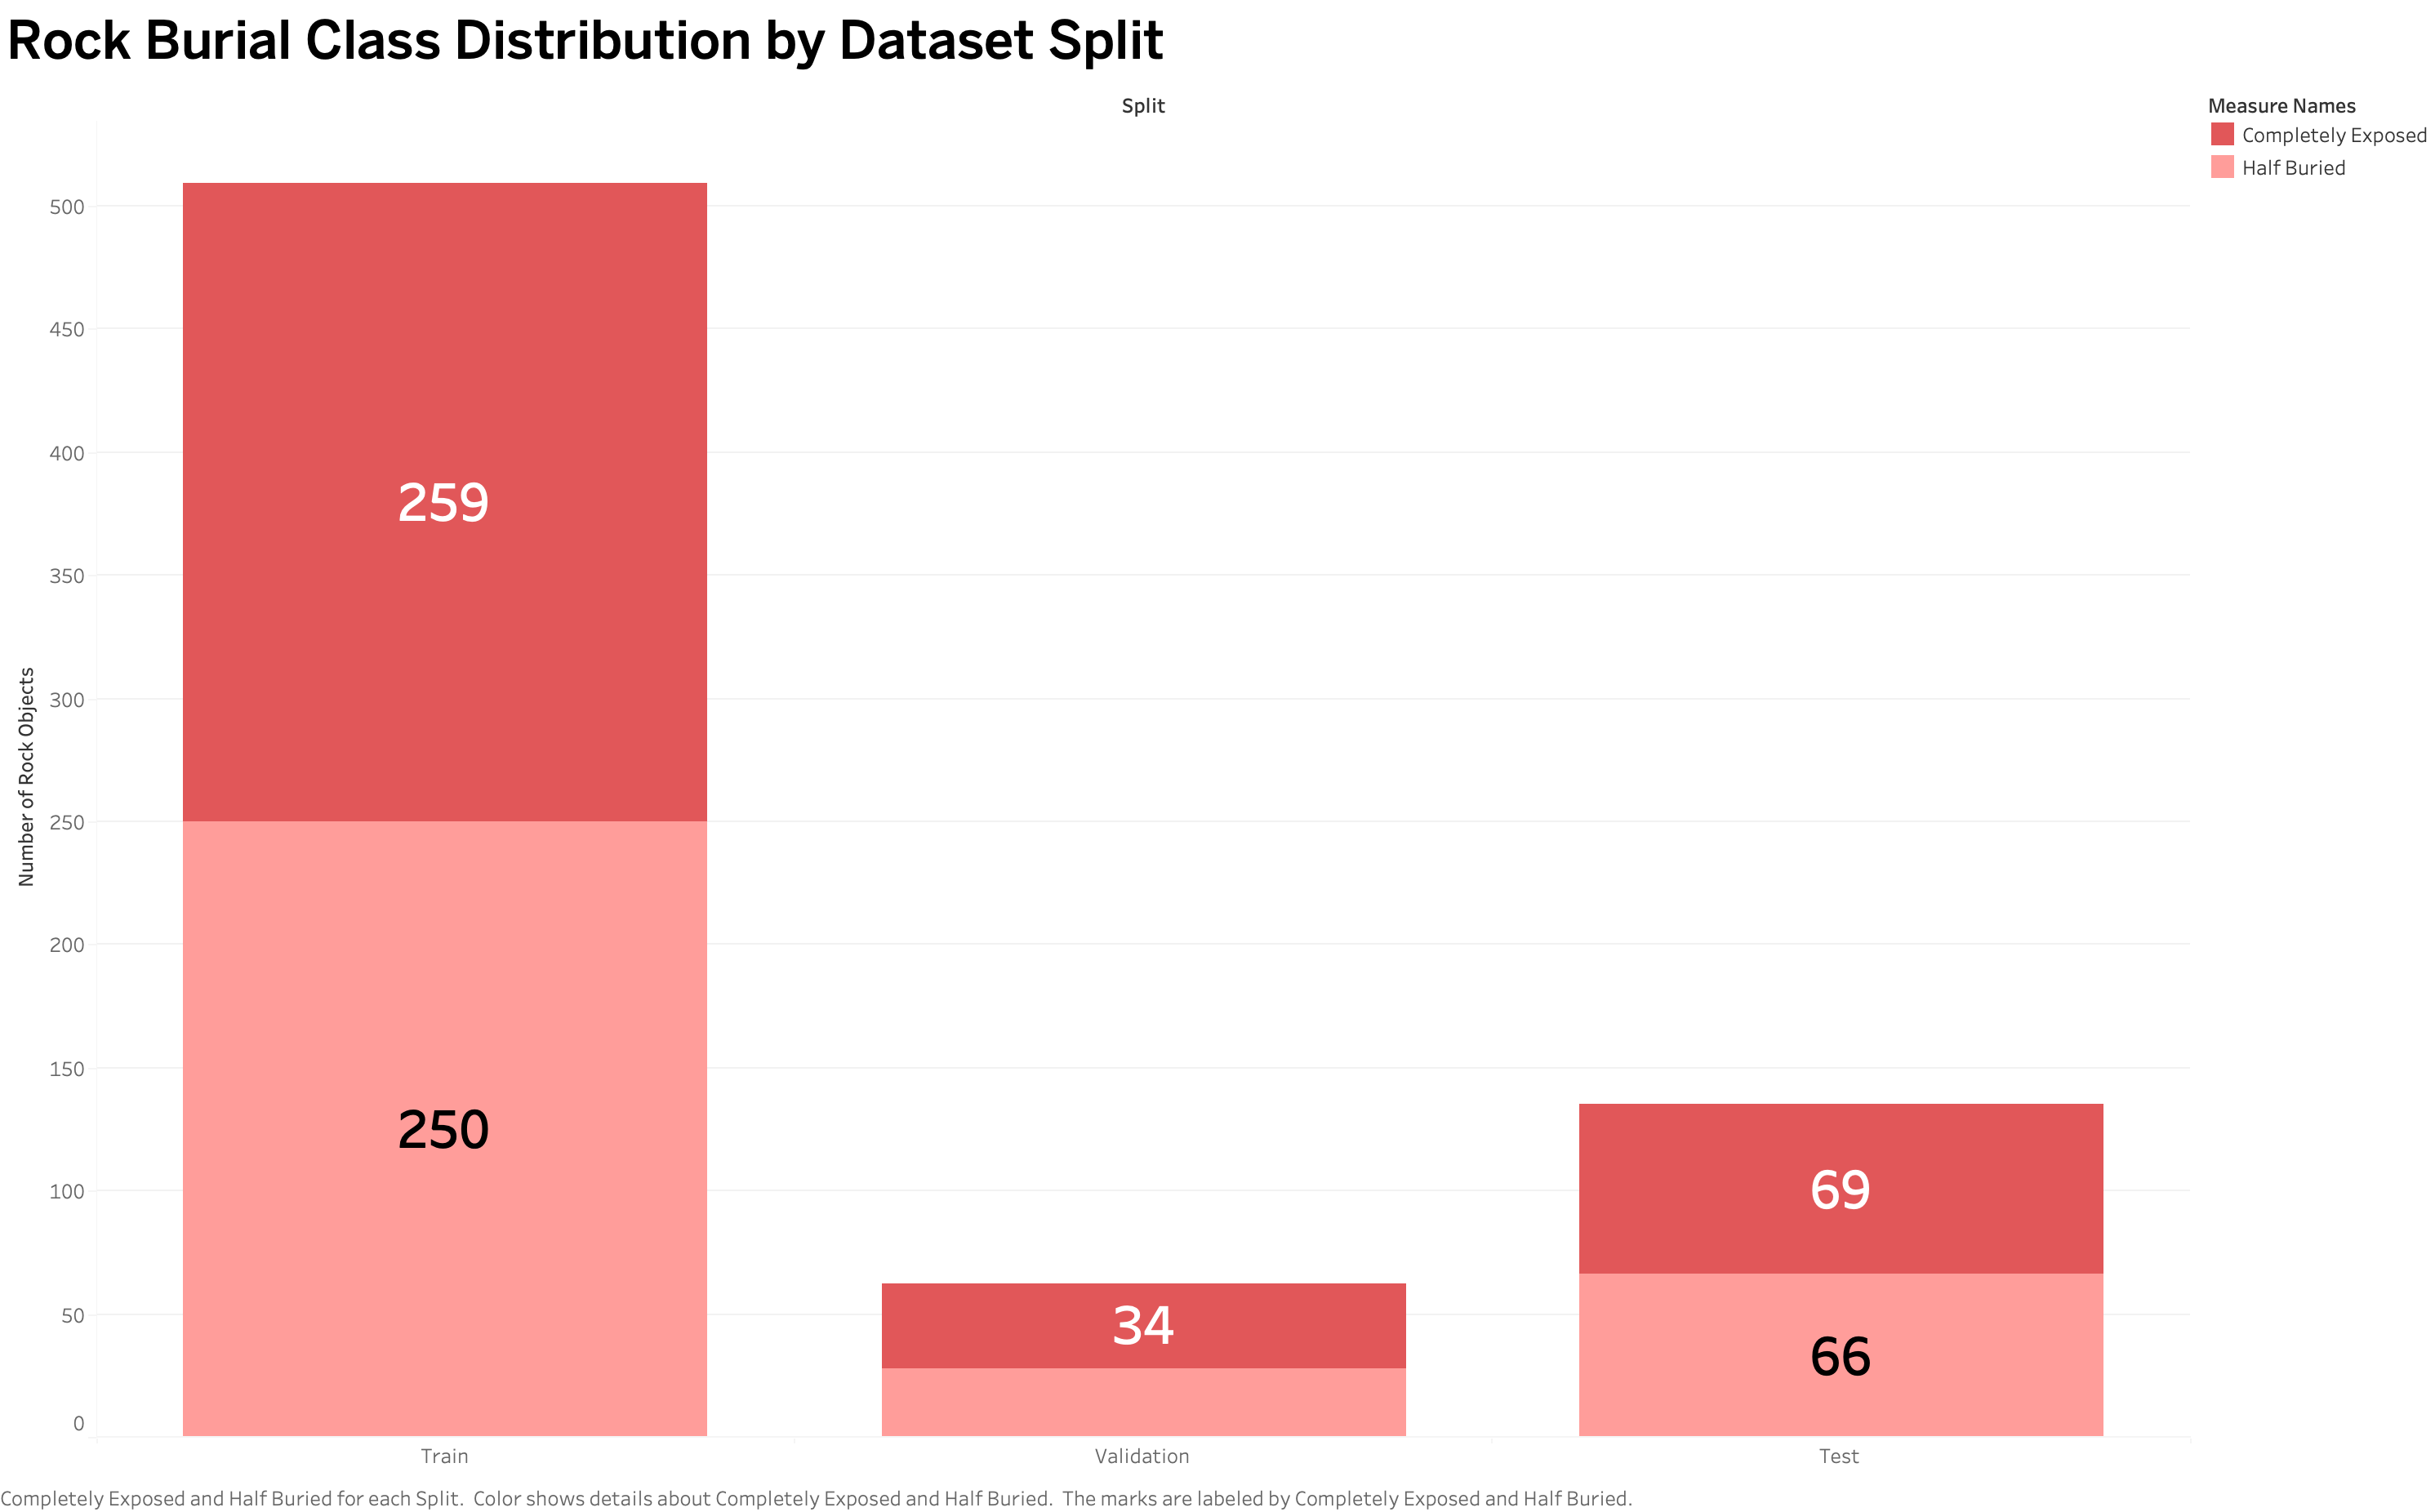
\includegraphics[width=\textwidth,height=4.2cm,keepaspectratio]{figures/figure_02.png}\\[2pt]
    {\tiny Figure 3.2: Class-level annotation counts across Train, Val, and Test splits.}
  \end{column}
\end{columns}
\end{frame}

% -------------------------------------------------------------
% SLIDE 8: Safe Augmentation
% -------------------------------------------------------------
\begin{frame}{Controlled Photometric Augmentation Expands Training to 2,191 Images}
\begin{columns}[T]
  \begin{column}{0.48\textwidth}
    \begin{block}{\small Safe Photometric Transformation}
      \small
      \begin{itemize}
        \item Each of the 313 training images received 6 photometric variants (+1,878 images), yielding \textbf{2,191 training images}.
        \item Training annotations expanded from 509 to \textbf{3,563 rock instances}.
        \item \textbf{Transforms:} Brightness/contrast shifts, gamma adjustments, and HSV colour jitter to simulate lighting changes.
        \item \textbf{Geometric Safety:} Extreme rotations/crops strictly avoided to maintain bounding box accuracy.
      \end{itemize}
    \end{block}
  \end{column}
  \begin{column}{0.48\textwidth}
    \centering
    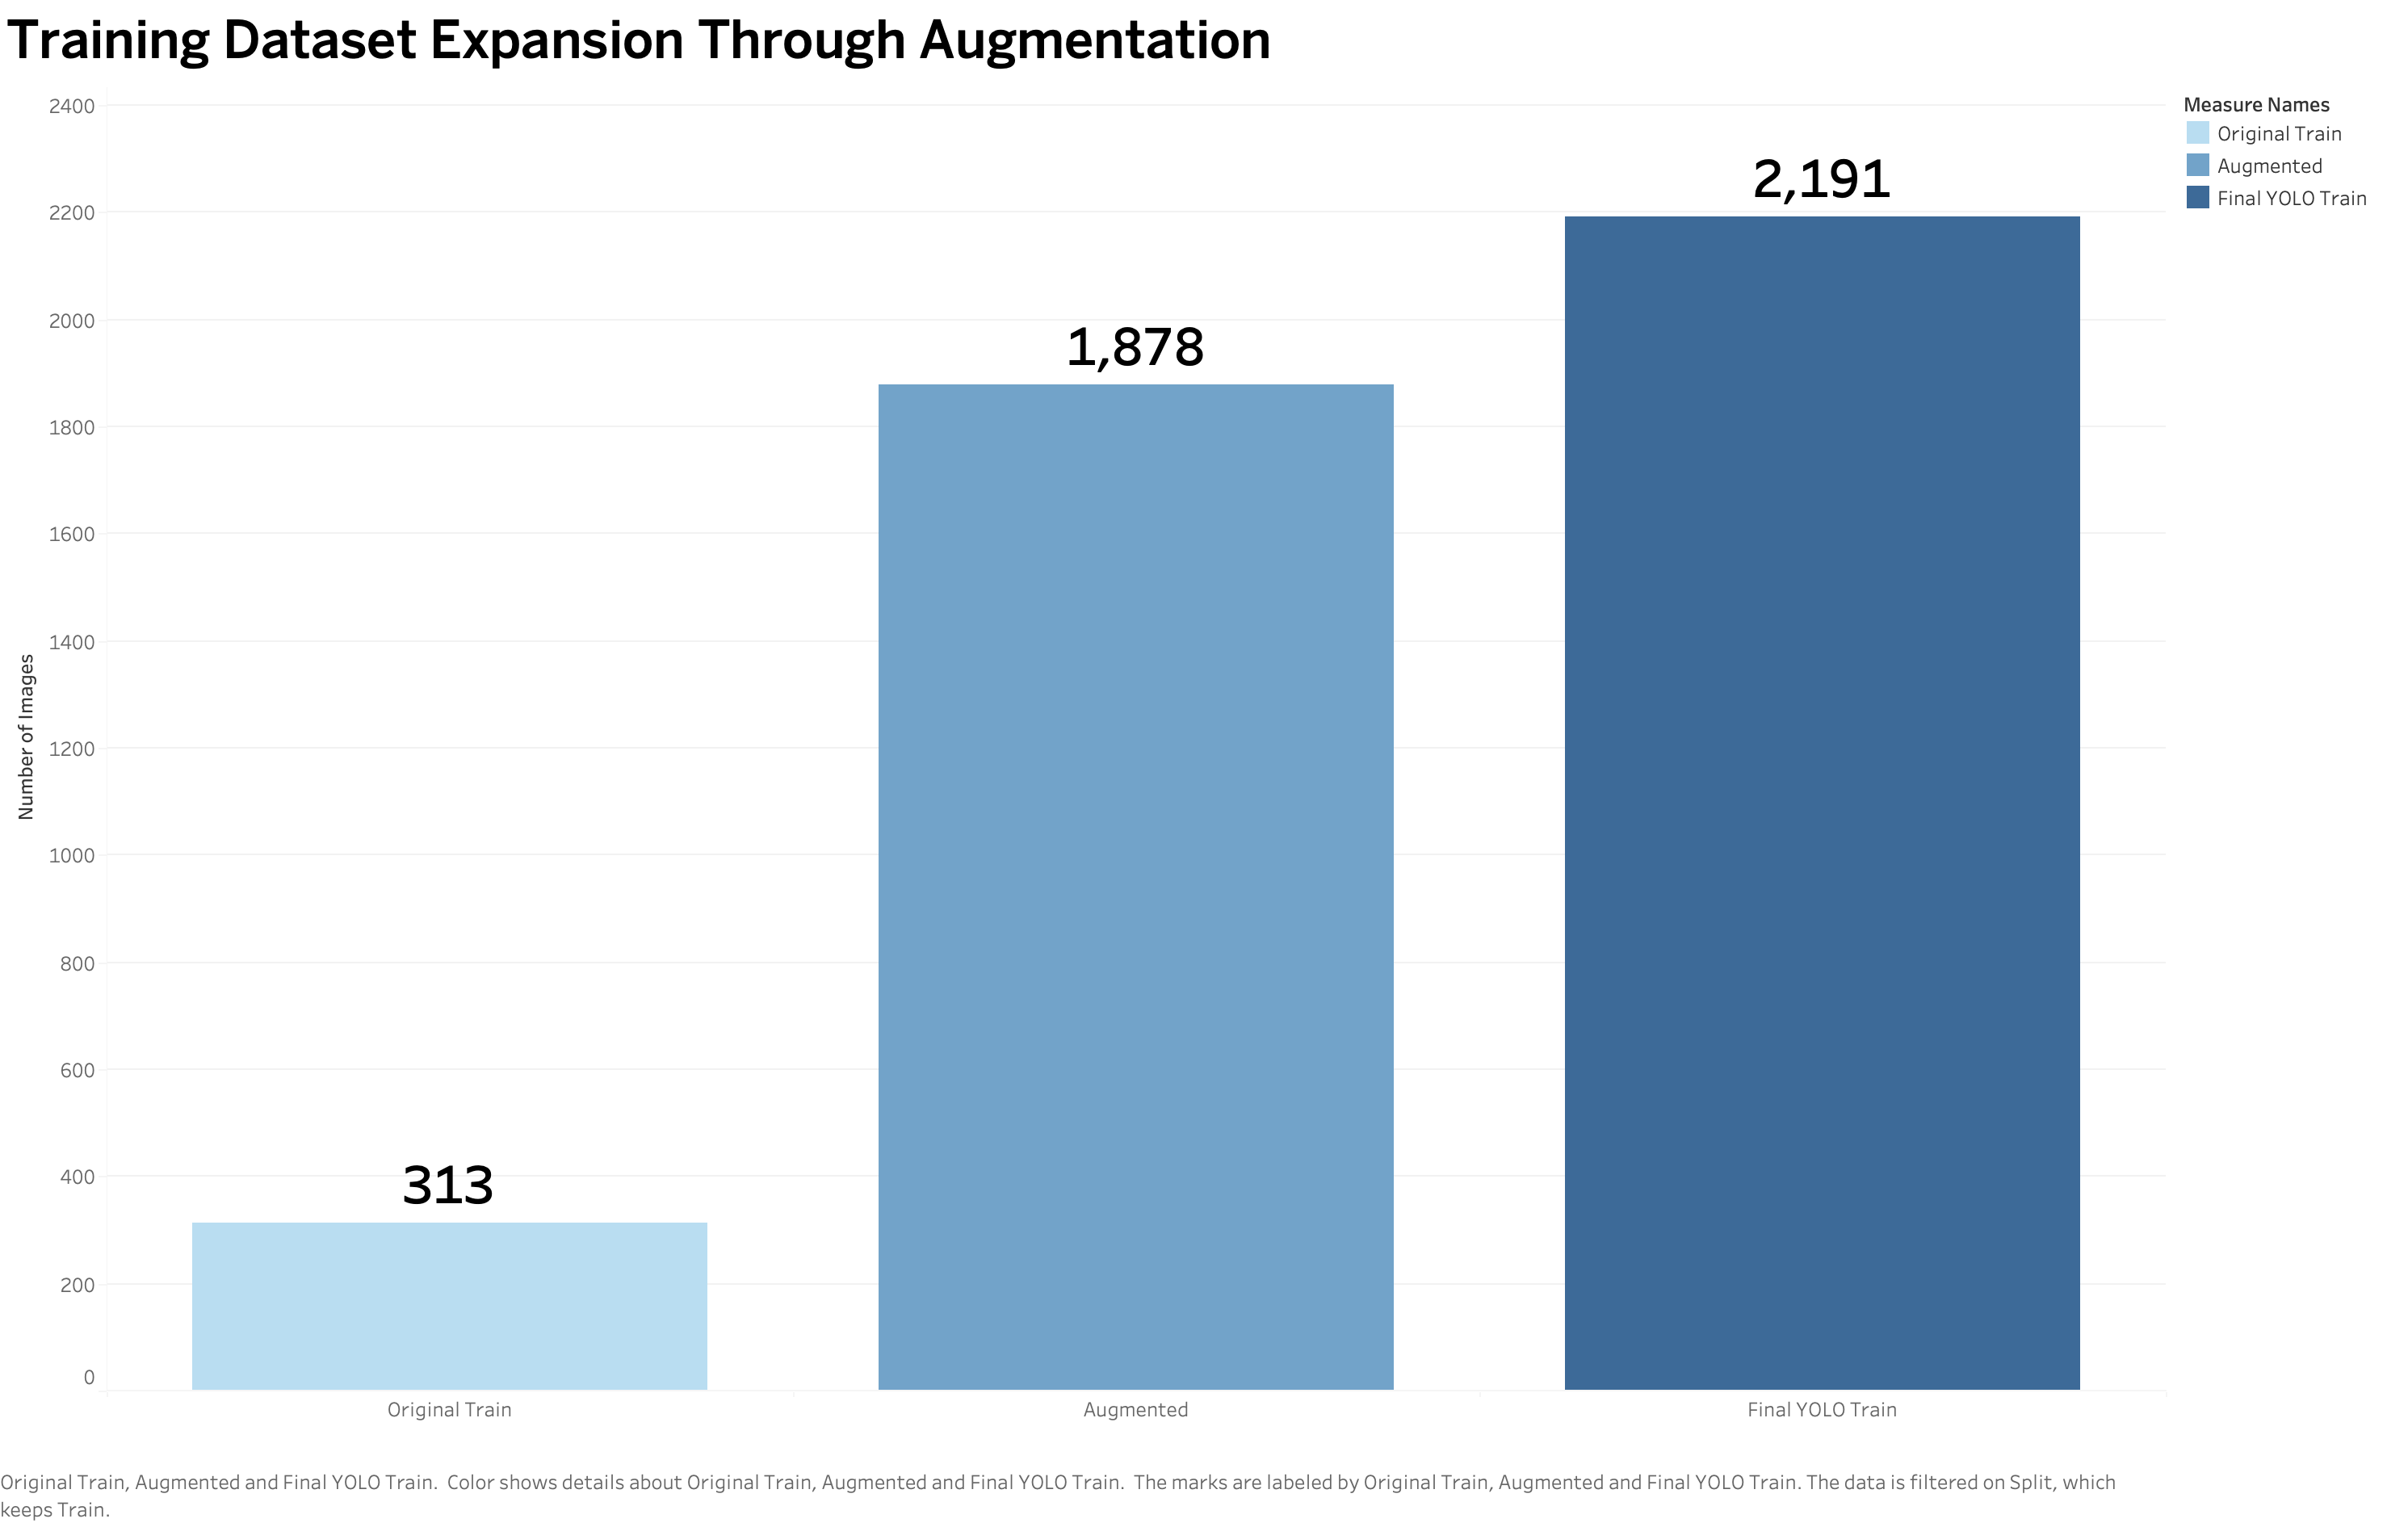
\includegraphics[width=\textwidth,height=4.2cm,keepaspectratio]{figures/figure_03.png}\\[2pt]
    {\tiny Figure 3.3: 7x expansion of the training partition from 313 to 2,191 images.}
  \end{column}
\end{columns}
\end{frame}

% -------------------------------------------------------------
% SLIDE 9: Single-Stage YOLO
% -------------------------------------------------------------
\section{Model Architecture}
\begin{frame}{Single-Stage YOLO Detects Location \& Burial Status Simultaneously}
\begin{columns}[T]
  \begin{column}{0.48\textwidth}
    \begin{block}{\small Why Single-Stage YOLO for Edge Vision?}
      \small
      \begin{itemize}
        \item Two-stage detectors (Faster R-CNN) require separate region proposal networks ($>800$~ms on ARM CPU).
        \item Single-stage YOLO predicts bounding boxes $[x, y, w, h]$ and class probabilities in a \textbf{single forward pass}.
        \item Modern anchor-free architecture adapts to irregular rock shapes and small objects without manual anchor tuning.
      \end{itemize}
    \end{block}
  \end{column}
  \begin{column}{0.48\textwidth}
    \begin{block}{\small Output Processing Pipeline}
      \small
      \begin{itemize}
        \item \textbf{Input:} $640\times640\times3$ RGB tensor.
        \item \textbf{Decoded Output:} 8,400 candidate anchor predictions.
        \item \textbf{Confidence Threshold:} Filtering scores $< 0.25$.
        \item \textbf{NMS:} IoU threshold $0.70$ removes duplicate detections.
        \item \textbf{Telemetry Output:} Box coordinates, class labels, inference latency, and aggregate rock counts per image.
      \end{itemize}
    \end{block}
  \end{column}
\end{columns}
\end{frame}

% -------------------------------------------------------------
% SLIDE 10: Controlled Candidate Training
% -------------------------------------------------------------
\section{Model Development}
\begin{frame}{Controlled Training of Lightweight YOLO Candidates}
\begin{columns}[T]
  \begin{column}{0.48\textwidth}
    \begin{block}{\small Experimental Setup}
      \small
      \begin{itemize}
        \item Evaluated three architectures: \textbf{YOLOv8n} (3.2M params), \textbf{YOLO11n} (2.6M params), and \textbf{YOLO11s} (9.4M params).
        \item \textbf{Identical Hyperparameters:} 20 epochs, AdamW optimiser, Cosine LR scheduler, batch size 32, AMP enabled.
        \item Pre-trained COCO transfer learning initialisation.
        \item Validation evaluation at 1024-pixel resolution.
      \end{itemize}
    \end{block}
  \end{column}
  \begin{column}{0.48\textwidth}
    \centering
    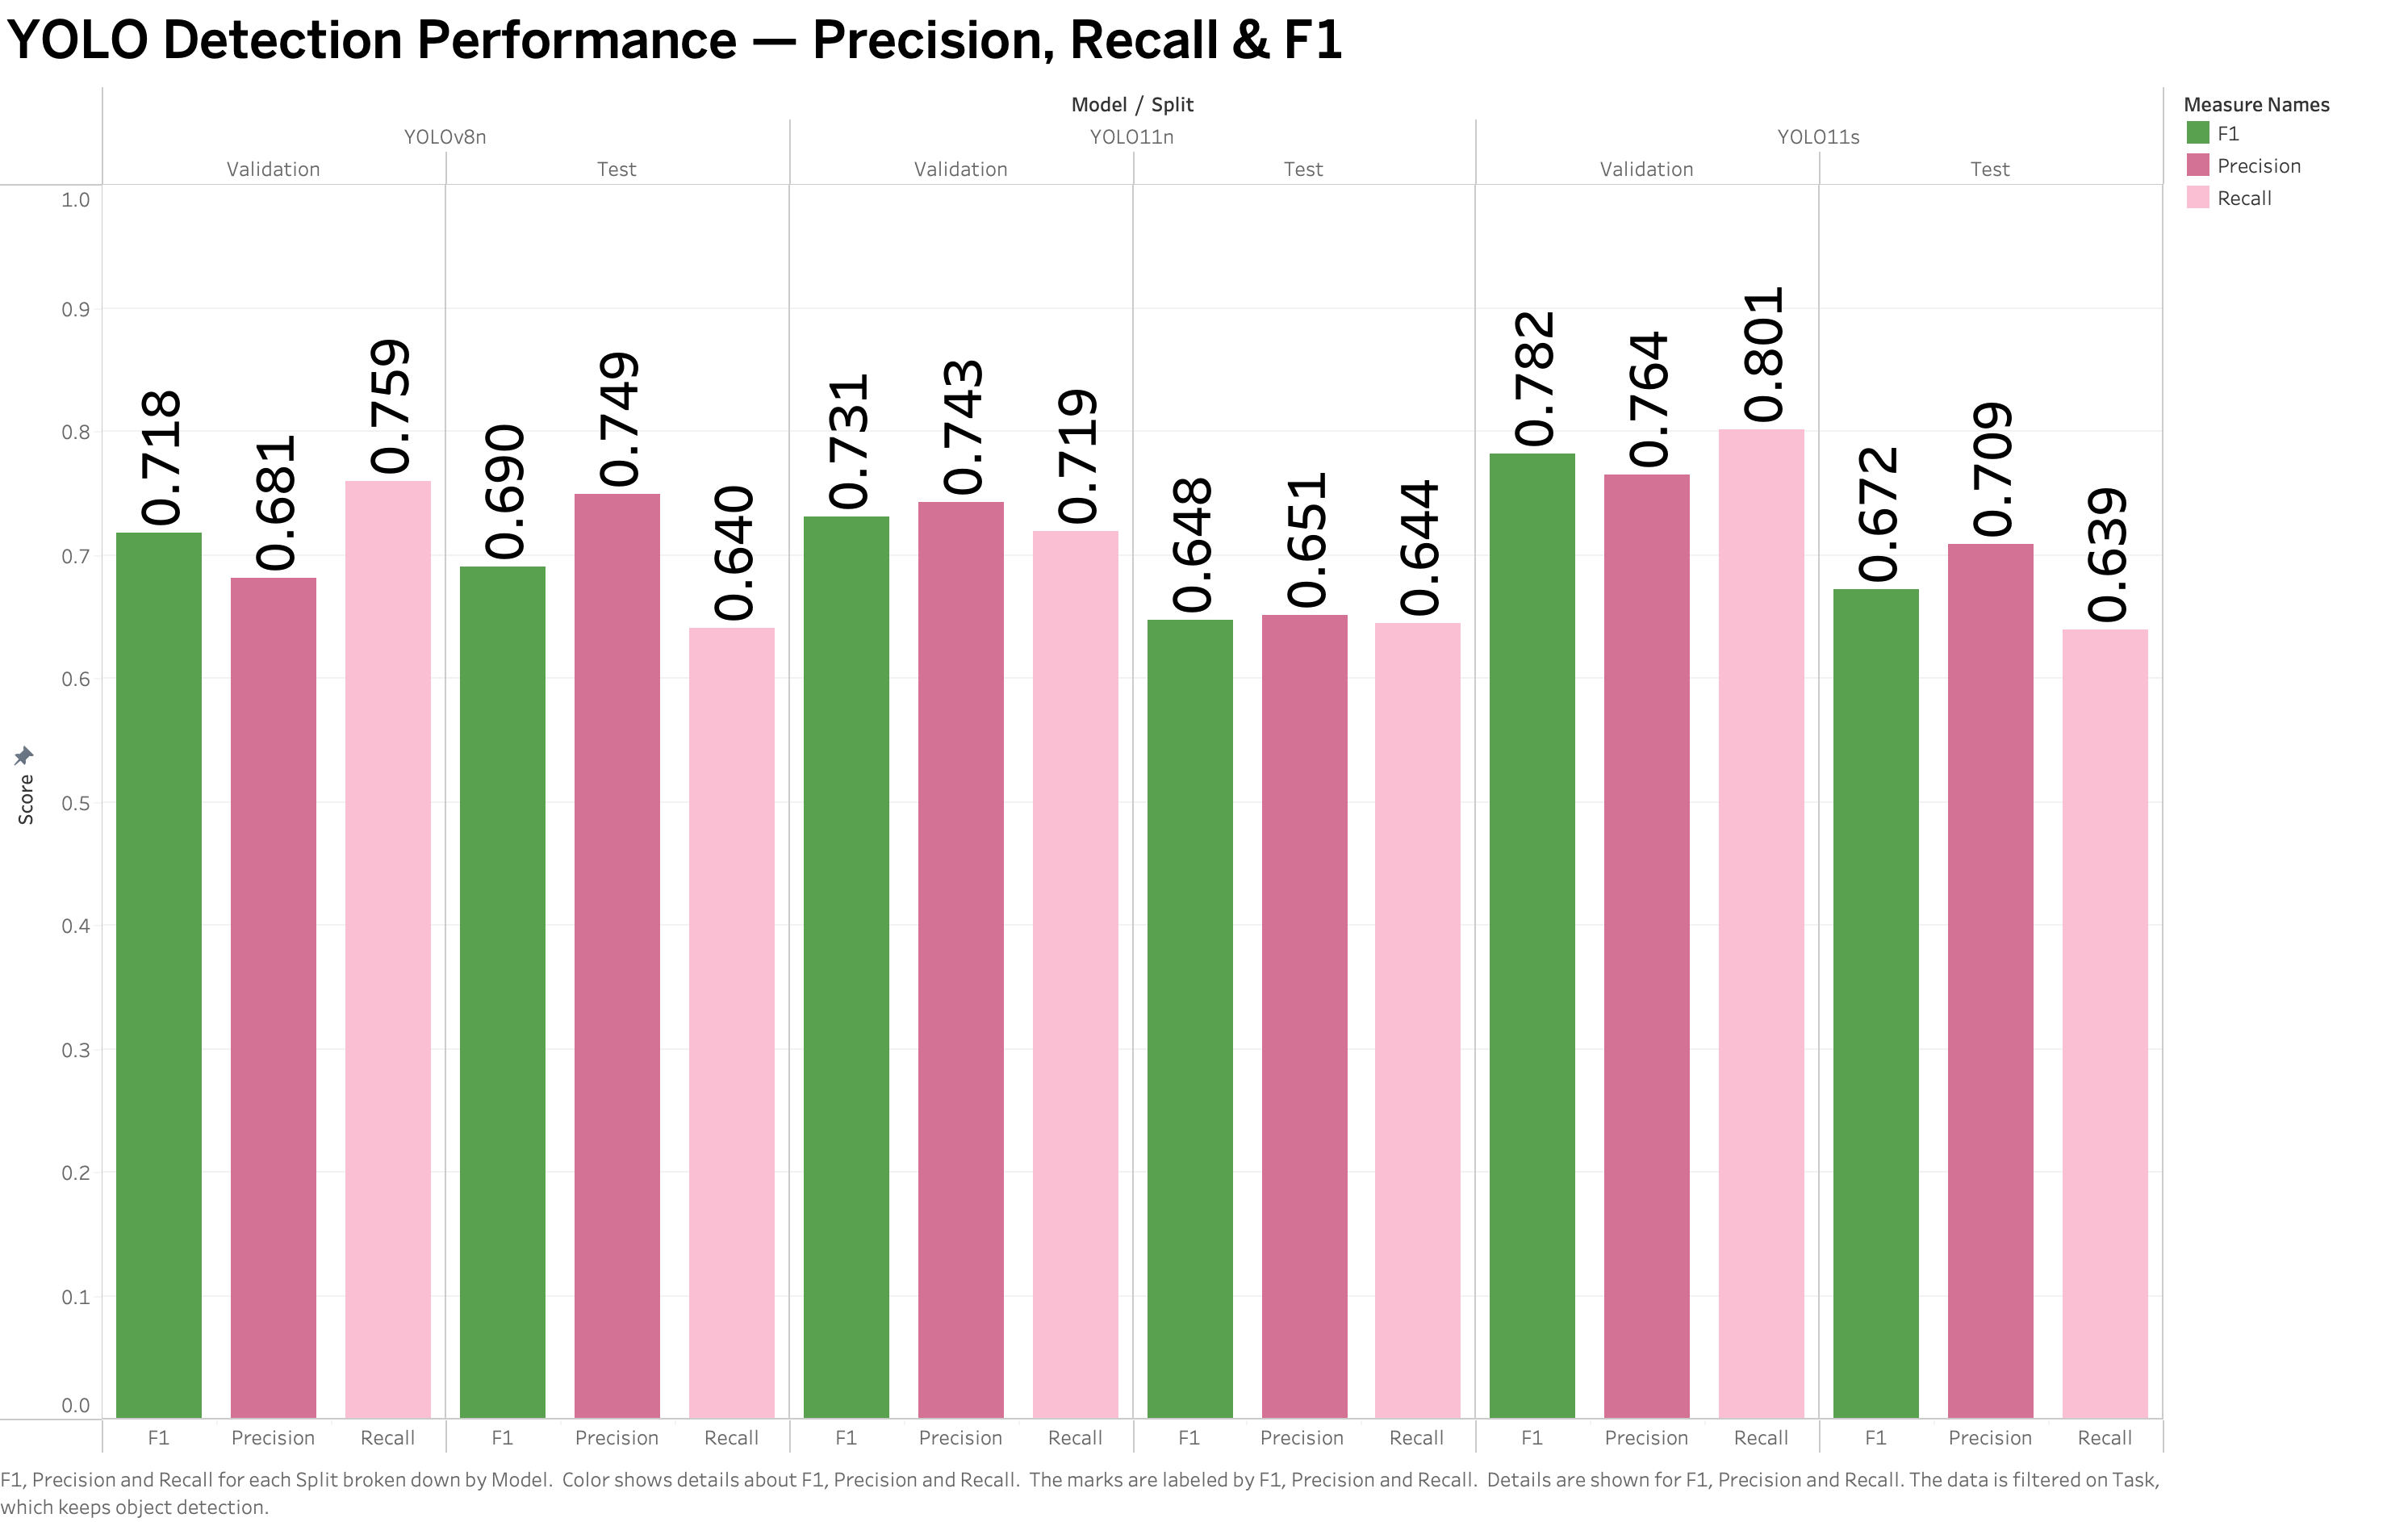
\includegraphics[width=\textwidth,height=4.2cm,keepaspectratio]{figures/figure_05.png}\\[2pt]
    {\tiny Figure 3.5: Precision, Recall, and F1 across candidate YOLO architectures.}
  \end{column}
\end{columns}
\end{frame}

% -------------------------------------------------------------
% SLIDE 11: Architecture Selection Criterion
% -------------------------------------------------------------
\begin{frame}{Predefined Primary Criterion: Validation mAP50–95}
\begin{columns}[T]
  \begin{column}{0.48\textwidth}
    \begin{block}{\small Rigorous Selection Standard}
      \small
      \begin{itemize}
        \item Architecture selection governed strictly by \textbf{Validation mAP50--95}.
        \item \textbf{Why mAP50--95 over mAP50?}
        \begin{itemize}
          \item mAP50 evaluates loose overlap (IoU $\ge 0.50$).
          \item mAP50--95 averages across IoU 0.50 to 0.95, strictly penalising poor bounding box localisation.
        \end{itemize}
        \item Accurate boundary estimation is vital for mechanical rock pickers to avoid striking stone edges.
      \end{itemize}
    \end{block}
  \end{column}
  \begin{column}{0.48\textwidth}
    \begin{block}{\small Candidate Validation Scores}
      \small
      \begin{table}
        \centering
        \footnotesize
        \begin{tabular}{|l|c|c|c|}
          \hline
          Model & F1 & mAP50 & mAP50--95 \\
          \hline
          \textbf{YOLOv8n} & 0.718 & 0.759 & \textbf{0.4288} \\
          \hline
          YOLO11n & 0.731 & 0.729 & 0.4002 \\
          \hline
          YOLO11s & \textbf{0.782} & \textbf{0.783} & 0.4107 \\
          \hline
        \end{tabular}
      \end{table}
      \vspace{-4pt}
      \textbf{Decision:} YOLOv8n selected based on the predefined primary criterion and compact 3.2M parameter size.
    \end{block}
  \end{column}
\end{columns}
\end{frame}

% -------------------------------------------------------------
% SLIDE 12: Detector Selection Result
% -------------------------------------------------------------
\begin{frame}{YOLOv8n Achieves Highest Validation Localisation Quality}
\begin{columns}[T]
  \begin{column}{0.48\textwidth}
    \begin{block}{\small Selection Summary}
      \small
      \begin{itemize}
        \item YOLOv8n achieved \textbf{mAP50--95 = 0.4288}, outperforming YOLO11n (0.4002, +7.1\%) and YOLO11s (0.4107, +4.4\%).
        \item Although YOLO11s scored slightly higher on F1 (0.782), its 9.4M parameter size tripled compute requirements.
        \item YOLOv8n provided the optimal balance of localisation precision and lightweight footprint.
        \item Checkpoint weights frozen for multi-format edge export.
      \end{itemize}
    \end{block}
  \end{column}
  \begin{column}{0.48\textwidth}
    \centering
    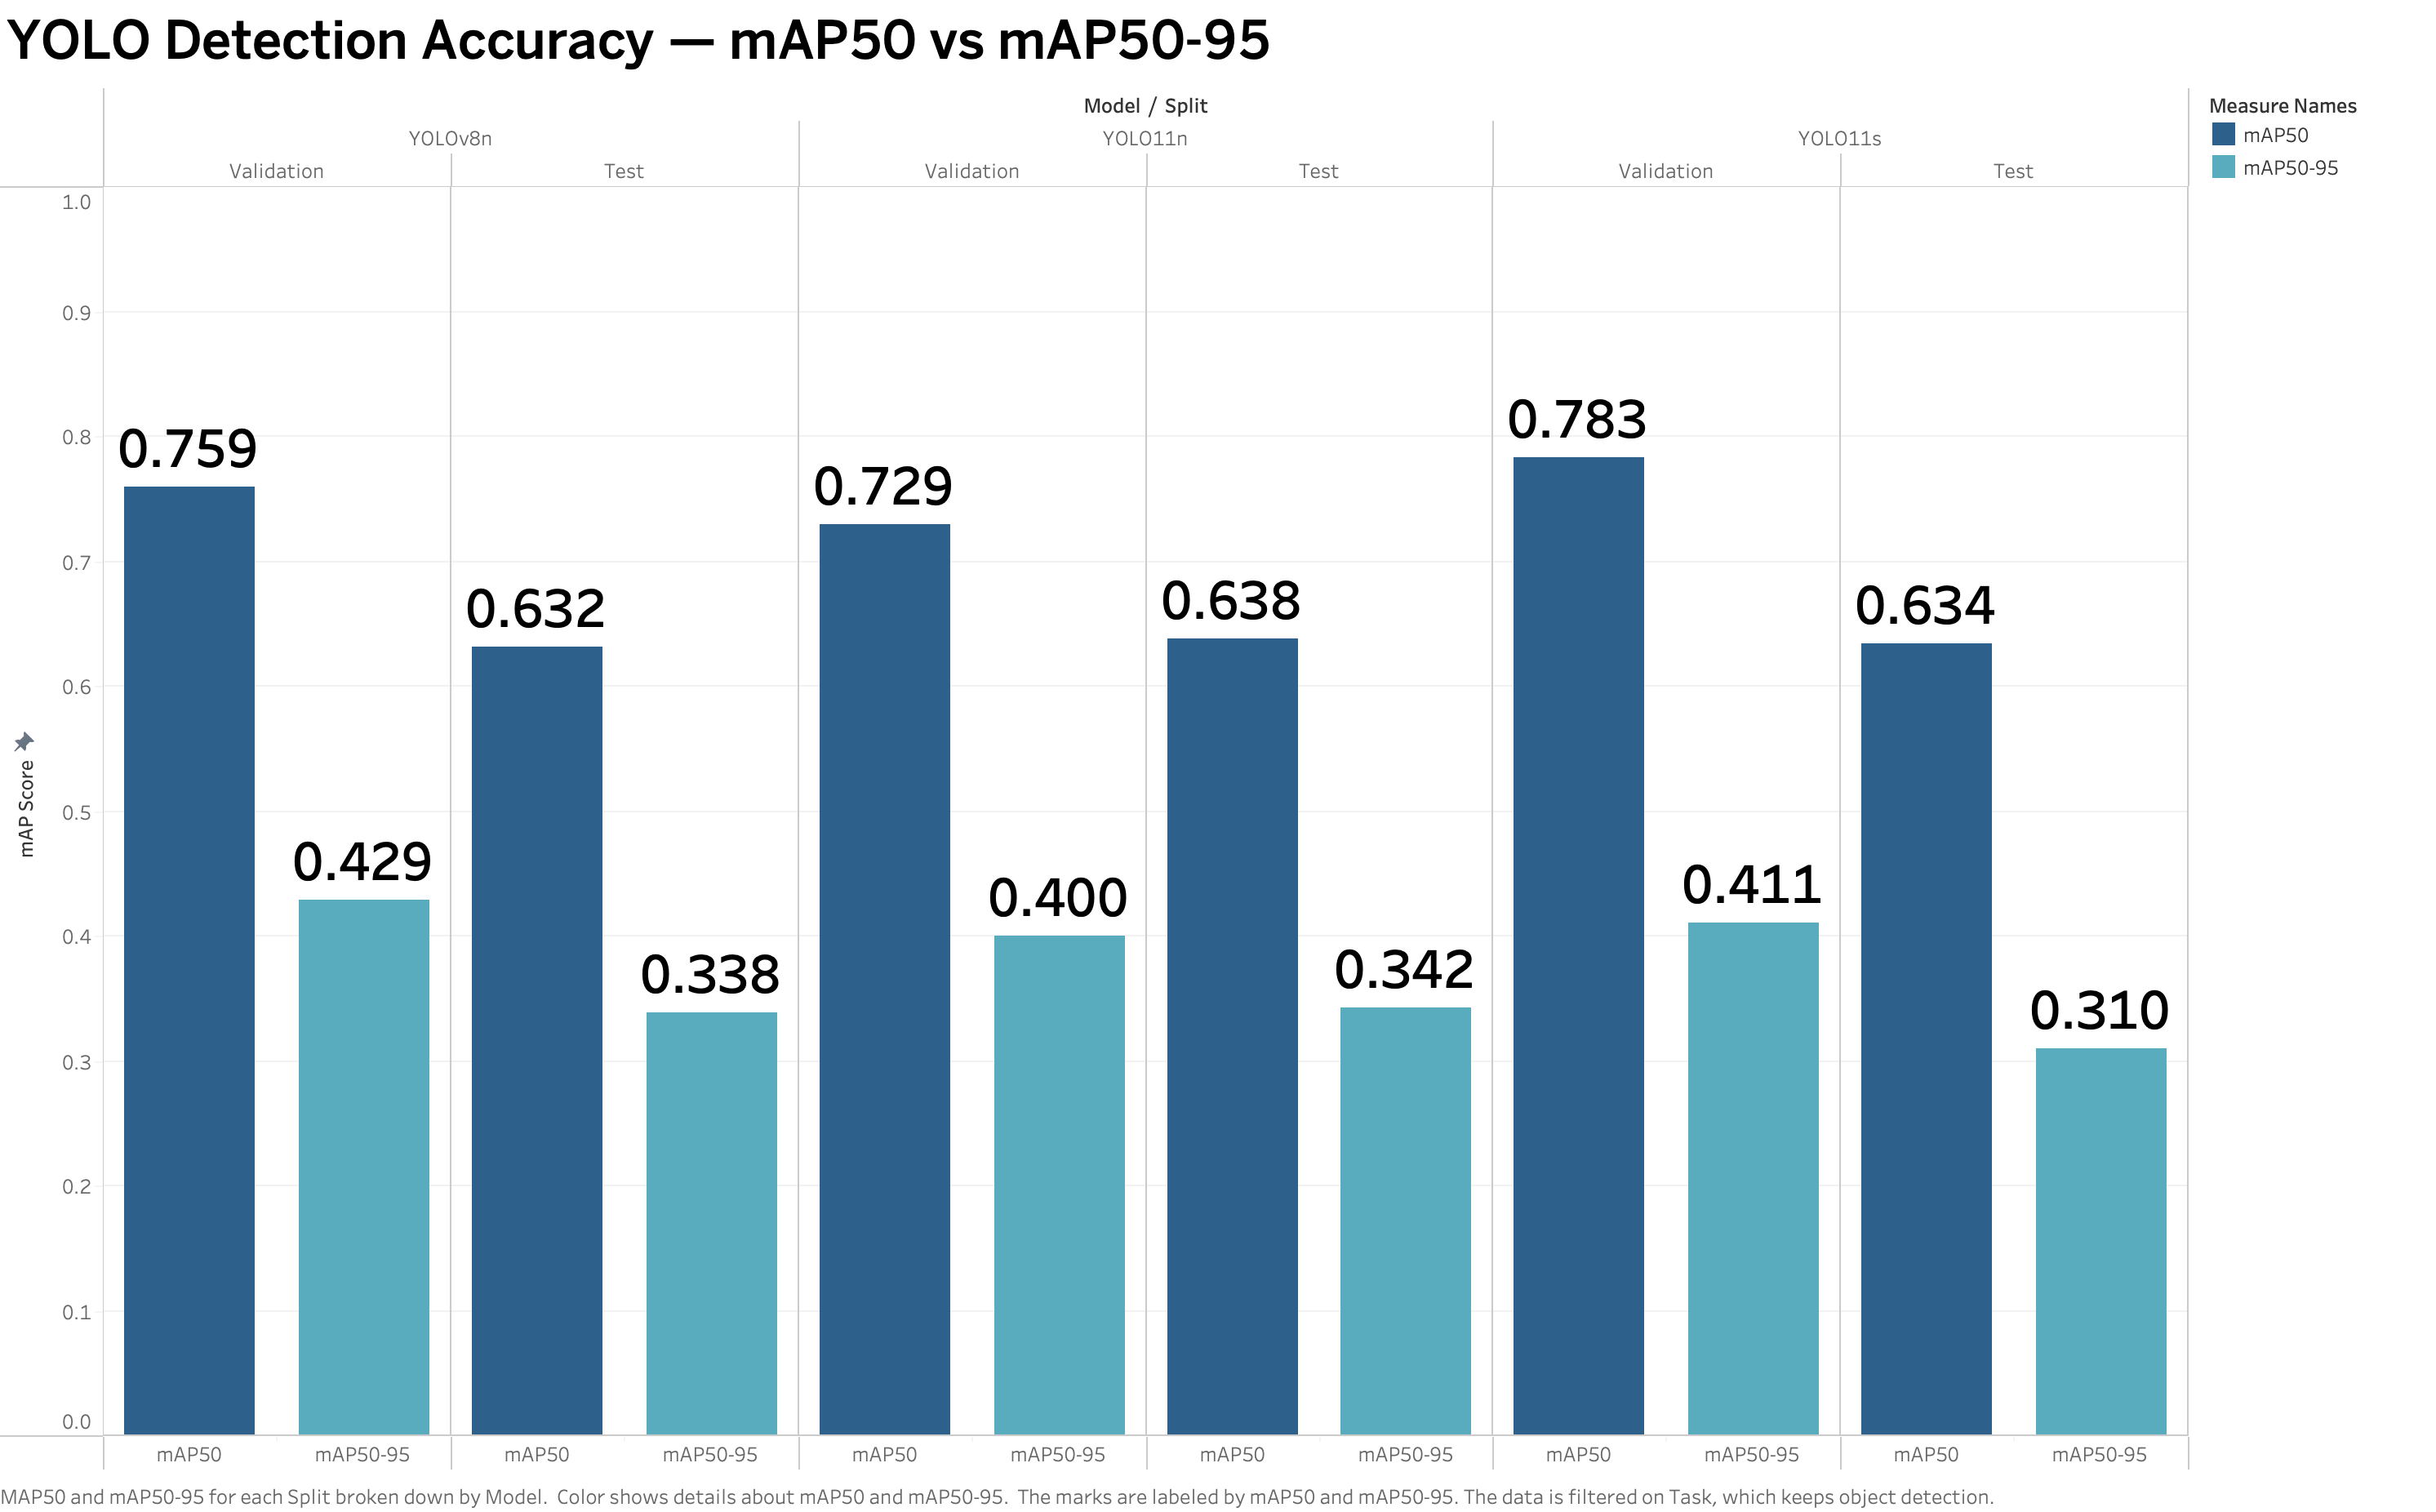
\includegraphics[width=\textwidth,height=4.2cm,keepaspectratio]{figures/figure_06.png}\\[2pt]
    {\tiny Figure 3.6: mAP50 and mAP50--95 on validation and test partitions.}
  \end{column}
\end{columns}
\end{frame}

% -------------------------------------------------------------
% SLIDE 13: Generalisation & Burial Difficulty
% -------------------------------------------------------------
\section{Model Diagnostics}
\begin{frame}{Class Breakdown Reveals Inherent Difficulty of Half-Buried Rocks}
\begin{columns}[T]
  \begin{column}{0.48\textwidth}
    \begin{block}{\small Class-Specific Asymmetry on Test Set}
      \small
      \begin{itemize}
        \item \textbf{Completely Exposed:} 64 / 69 rocks detected correctly (\textbf{92.8\% operational accuracy}).
        \item \textbf{Half-Buried:} Only 23 / 66 rocks detected correctly (\textbf{34.8\% operational accuracy}).
        \item \textbf{Failure Causes:}
        \begin{itemize}
          \item Gradual surface-to-soil boundary blending.
          \item Partial soil occlusion and shadow contours.
          \item Absence of continuous high-contrast edges.
        \end{itemize}
      \end{itemize}
    \end{block}
  \end{column}
  \begin{column}{0.48\textwidth}
    \begin{block}{\small Operational Implication}
      \small
      \begin{itemize}
        \item Exposed rocks are detected with $>90\%$ reliability for fast surface sweeps.
        \item Half-buried rocks require deeper penetration and higher actuation force; classification errors risk machinery jams.
        \item 2D RGB imagery alone reaches a performance ceiling; future 3D sensing is recommended.
      \end{itemize}
    \end{block}
  \end{column}
\end{columns}
\end{frame}

% -------------------------------------------------------------
% SLIDE 14: Auxiliary CLIP Investigation
% -------------------------------------------------------------
\begin{frame}{CLIP Enhances Crop Classification but Lacks Native Localisation}
\begin{columns}[T]
  \begin{column}{0.48\textwidth}
    \begin{block}{\small Zero-Shot vs Fine-Tuned CLIP (ViT-B/32)}
      \small
      \begin{itemize}
        \item Investigated whether foundation vision-language models could improve burial classification on cropped rock chips.
        \item \textbf{Zero-Shot CLIP:} 50.4\% accuracy (chance level between exposed vs buried).
        \item \textbf{Fine-Tuned CLIP:} \textbf{80.0\% accuracy} on cropped rock chips.
        \item Demonstrates strong semantic feature representations once fine-tuned on agricultural data.
      \end{itemize}
    \end{block}
  \end{column}
  \begin{column}{0.48\textwidth}
    \begin{block}{\small Why CLIP Was Not Deployed to Edge}
      \small
      \begin{itemize}
        \item CLIP is a crop classifier, \textbf{not an object detector}; requires a separate detector to provide bounding boxes.
        \item Two-stage pipeline doubles complexity.
        \item ViT-B/32 requires $\sim 350$~MB RAM and $\sim 850$~ms latency per crop on Raspberry Pi 5 --- far too slow for real-time control.
      \end{itemize}
    \end{block}
  \end{column}
\end{columns}
\end{frame}

% -------------------------------------------------------------
% SLIDE 15: Edge Inference Pipeline
% -------------------------------------------------------------
\section{Edge Pipeline}
\begin{frame}{End-to-End Edge Pipeline: Letterboxing to Count Telemetry}
\begin{columns}[T]
  \begin{column}{0.48\textwidth}
    \begin{block}{\small Data Flow on Raspberry Pi}
      \small
      \begin{enumerate}
        \item \textbf{Letterboxing:} $640\times640$ with aspect-ratio preservation and fill value 114.
        \item \textbf{Tensor Conversion:} RGB normalization $[0, 1]$ and NCHW formatting.
        \item \textbf{Engine Inference:} Multi-backend forward pass (PyTorch, TFLite, NCNN, ONNX).
        \item \textbf{Post-Processing:} Threshold filtering ($\ge 0.25$) and NMS (IoU 0.70).
        \item \textbf{Output Telemetry:} Bounding boxes, labels, FPS, and rock count MAE.
      \end{enumerate}
    \end{block}
  \end{column}
  \begin{column}{0.48\textwidth}
    \begin{block}{\small Rock Counting Mean Absolute Error (MAE)}
      \small
      \begin{itemize}
        \item \textbf{PyTorch FP32:} $\text{MAE} = 0.600$ rocks/image
        \item \textbf{TFLite FP32:} $\text{MAE} = 0.600$ rocks/image
        \item \textbf{TFLite INT8:} $\text{MAE} = 0.633$ rocks/image (+0.033 error delta)
        \item \textbf{NCNN FP32:} $\text{MAE} = 0.600$ rocks/image
        \item \textbf{NCNN FP16:} $\text{MAE} = 0.611$ rocks/image
      \end{itemize}
      \vspace{2pt}
      INT8 quantisation retains excellent rock-counting fidelity across test images.
    \end{block}
  \end{column}
\end{columns}
\end{frame}

% -------------------------------------------------------------
% SLIDE 16: Qualitative Error Analysis
% -------------------------------------------------------------
\begin{frame}{Qualitative Failure Modes: Soil Clods \& Occlusion Boundaries}
\begin{columns}[T]
  \begin{column}{0.48\textwidth}
    \begin{block}{\small Systematic Error Patterns}
      \small
      \begin{itemize}
        \item \textbf{False Positives (Soil Clods):} Dry, crusted soil clumps frequently exhibit convex contours and shadow gradients mimicking small rocks.
        \item \textbf{False Negatives (Deep Burial):} Rocks with $<20\%$ surface exposure blend into tillage patterns.
        \item \textbf{Boundary Oscillation:} Stones with $\sim 50\%$ burial fluctuate between exposed and half-buried classes.
      \end{itemize}
    \end{block}
  \end{column}
  \begin{column}{0.48\textwidth}
    \begin{block}{\small Diagnostic Insights}
      \small
      \begin{itemize}
        \item \textbf{Illumination Robustness:} Photometric augmentation successfully prevented false alarms under harsh direct sunlight.
        \item \textbf{Scale Sensitivity:} Rocks $<30$ pixels across exhibit lower confidence; $640\times640$ represents the optimal speed-resolution trade-off.
        \item Suggests integrating 3D surface depth profiling in future tractor hardware revisions.
      \end{itemize}
    \end{block}
  \end{column}
\end{columns}
\end{frame}

% -------------------------------------------------------------
% SLIDE 17: Edge Preparation
% -------------------------------------------------------------
\section{Edge Methodology}
\begin{frame}{Preparation of Frozen Checkpoint \& Calibration Set}
\begin{columns}[T]
  \begin{column}{0.48\textwidth}
    \begin{block}{\small Checkpoint \& Calibration Design}
      \small
      \begin{itemize}
        \item Master YOLOv8n weights frozen into \texttt{best.pt} (6.2~MB).
        \item \textbf{INT8 Calibration Dataset:}
        \begin{itemize}
          \item Extracted 200 original training images containing 304 rock objects.
          \item Balanced at \textbf{152 exposed and 152 half-buried} instances.
          \item Computed static scale factor $S$ and zero-point $Z$ without backpropagation.
        \end{itemize}
        \item Zero test data observed during calibration.
      \end{itemize}
    \end{block}
  \end{column}
  \begin{column}{0.48\textwidth}
    \begin{block}{\small Affine Quantisation Formula}
      \small
      \begin{equation*}
        q = \text{round}\left(\frac{r}{S}\right) + Z
      \end{equation*}
      \begin{itemize}
        \item $r$: 32-bit floating point weight/activation.
        \item $q$: 8-bit signed integer $[-128, 127]$.
        \item $S$: positive real scale factor; $Z$: integer zero point.
        \item Unlocks ARM NEON integer dot-product SIMD instructions for massive edge speedups.
      \end{itemize}
    \end{block}
  \end{column}
\end{columns}
\end{frame}

% -------------------------------------------------------------
% SLIDE 18: Six Exported Representations
% -------------------------------------------------------------
\begin{frame}{Six Deployment Representations Span FP32, FP16 \& INT8}
\begin{columns}[T]
  \begin{column}{0.48\textwidth}
    \begin{block}{\small Evaluated Edge Representations}
      \small
      \begin{itemize}
        \item \textbf{PyTorch FP32 (6.2 MB):} Native baseline runtime.
        \item \textbf{TorchScript FP32 (12.3 MB):} JIT-compiled PyTorch IR.
        \item \textbf{ONNX FP32 (12.2 MB):} Open Neural Network Exchange.
        \item \textbf{TFLite FP32 (12.0 MB):} TensorFlow Lite float engine.
        \item \textbf{TFLite INT8 (3.3 MB):} 8-bit quantized flatbuffer (\textbf{--73\% file size}).
        \item \textbf{NCNN FP32 (12.1 MB) \& FP16 (6.1 MB):} High-performance mobile ARM engine.
      \end{itemize}
    \end{block}
  \end{column}
  \begin{column}{0.48\textwidth}
    \begin{block}{\small Multi-Format Scope}
      \small
      \begin{itemize}
        \item All six representations exported from identical frozen weights.
        \item File sizes span from 12.3~MB down to 3.3~MB.
        \item Enables rigorous cross-comparison across runtime engines (PyTorch vs TFLite vs NCNN vs ONNX) and numerical precisions (FP32 vs FP16 vs INT8).
      \end{itemize}
    \end{block}
  \end{column}
\end{columns}
\end{frame}

% -------------------------------------------------------------
% SLIDE 19: Raspberry Pi 5 Testbed
% -------------------------------------------------------------
\begin{frame}{Hardware Testbed: Raspberry Pi 5 (8GB) in CPU-Only Mode}
\begin{columns}[T]
  \begin{column}{0.48\textwidth}
    \begin{block}{\small Raspberry Pi 5 Specifications}
      \small
      \begin{itemize}
        \item \textbf{SoC:} Broadcom BCM2712 quad-core ARM Cortex-A76 @ 2.4 GHz.
        \item \textbf{Memory:} 8 GB LPDDR4X SDRAM.
        \item \textbf{Power:} Official 27W (5.1V / 5.0A) USB-C power supply.
        \item \textbf{OS:} Debian GNU/Linux 13 (Trixie), 64-bit kernel.
        \item \textbf{Cooling:} Passive heatsink only (No Active Cooler) to simulate enclosed tractor equipment boxes.
        \item \textbf{Stack:} Python 3.13.5, Ultralytics 8.4.115, ONNX Runtime 1.28.0, OpenCV 5.0.0.
      \end{itemize}
    \end{block}
  \end{column}
  \begin{column}{0.48\textwidth}
    \begin{block}{\small Experimental Protocol Controls}
      \small
      \begin{itemize}
        \item Headless OS environment without desktop GUI jitter.
        \item Batch size = 1 strictly enforced (live video simulation).
        \item Hardware telemetry: psutil and vcgencmd polled at 10~ms intervals for CPU load, RSS memory, and SoC core temperature.
      \end{itemize}
    \end{block}
  \end{column}
\end{columns}
\end{frame}

% -------------------------------------------------------------
% SLIDE 20: Dual Testing Protocol
% -------------------------------------------------------------
\begin{frame}{Dual Testing Protocol: Fixed Benchmark \& Continuous Endurance}
\begin{columns}[T]
  \begin{column}{0.48\textwidth}
    \begin{block}{\small Phase 1: Canonical Fixed Benchmark}
      \small
      \begin{itemize}
        \item 3 warmup inferences to stabilize cache and JIT execution.
        \item 90 timed sequential inferences over held-out test set.
        \item Measures per-frame latency, median FPS, CPU \%, peak RAM, mAP50, mAP50--95, and Count MAE.
      \end{itemize}
    \end{block}
  \end{column}
  \begin{column}{0.48\textwidth}
    \begin{block}{\small Phase 2: Continuous Endurance Test}
      \small
      \begin{itemize}
        \item 900 consecutive inferences (10 passes of the 90-image test set).
        \item Tests memory leak accumulation, thermal throttling, and runtime stability under prolonged execution.
        \item \textbf{Insight:} Models can pass a 90-image benchmark but crash after 20 minutes in field conditions.
      \end{itemize}
    \end{block}
  \end{column}
\end{columns}
\end{frame}

% -------------------------------------------------------------
% SLIDE 21: Latency & Throughput Results (THE WINNER)
% -------------------------------------------------------------
\section{Evaluation Results}
\begin{frame}{TFLite INT8 Delivers 22.62 FPS --- 9.01x Speedup over PyTorch}
\begin{columns}[T]
  \begin{column}{0.48\textwidth}
    \begin{block}{\small Canonical Runtime Latency \& Throughput}
      \small
      \begin{itemize}
        \item \textbf{PyTorch FP32:} 397.48 ms \textbar\ 2.52 FPS (Baseline)
        \item \textbf{TFLite FP32:} 143.70 ms \textbar\ 6.95 FPS ($2.77\times$ speedup)
        \item \textbf{NCNN FP32:} 75.09 ms \textbar\ 13.26 FPS ($5.29\times$ speedup)
        \item \textbf{NCNN FP16:} 72.31 ms \textbar\ 13.82 FPS ($5.49\times$ speedup)
        \item \textbf{TFLite INT8 (WINNER):} \textbf{44.13 ms \textbar\ 22.62 FPS ($9.01\times$ speedup!)}
      \end{itemize}
      \vspace{2pt}
      TFLite INT8 is the \textbf{only} representation that exceeds the 20 FPS threshold required for real-time field operations.
    \end{block}
  \end{column}
  \begin{column}{0.48\textwidth}
    \centering
    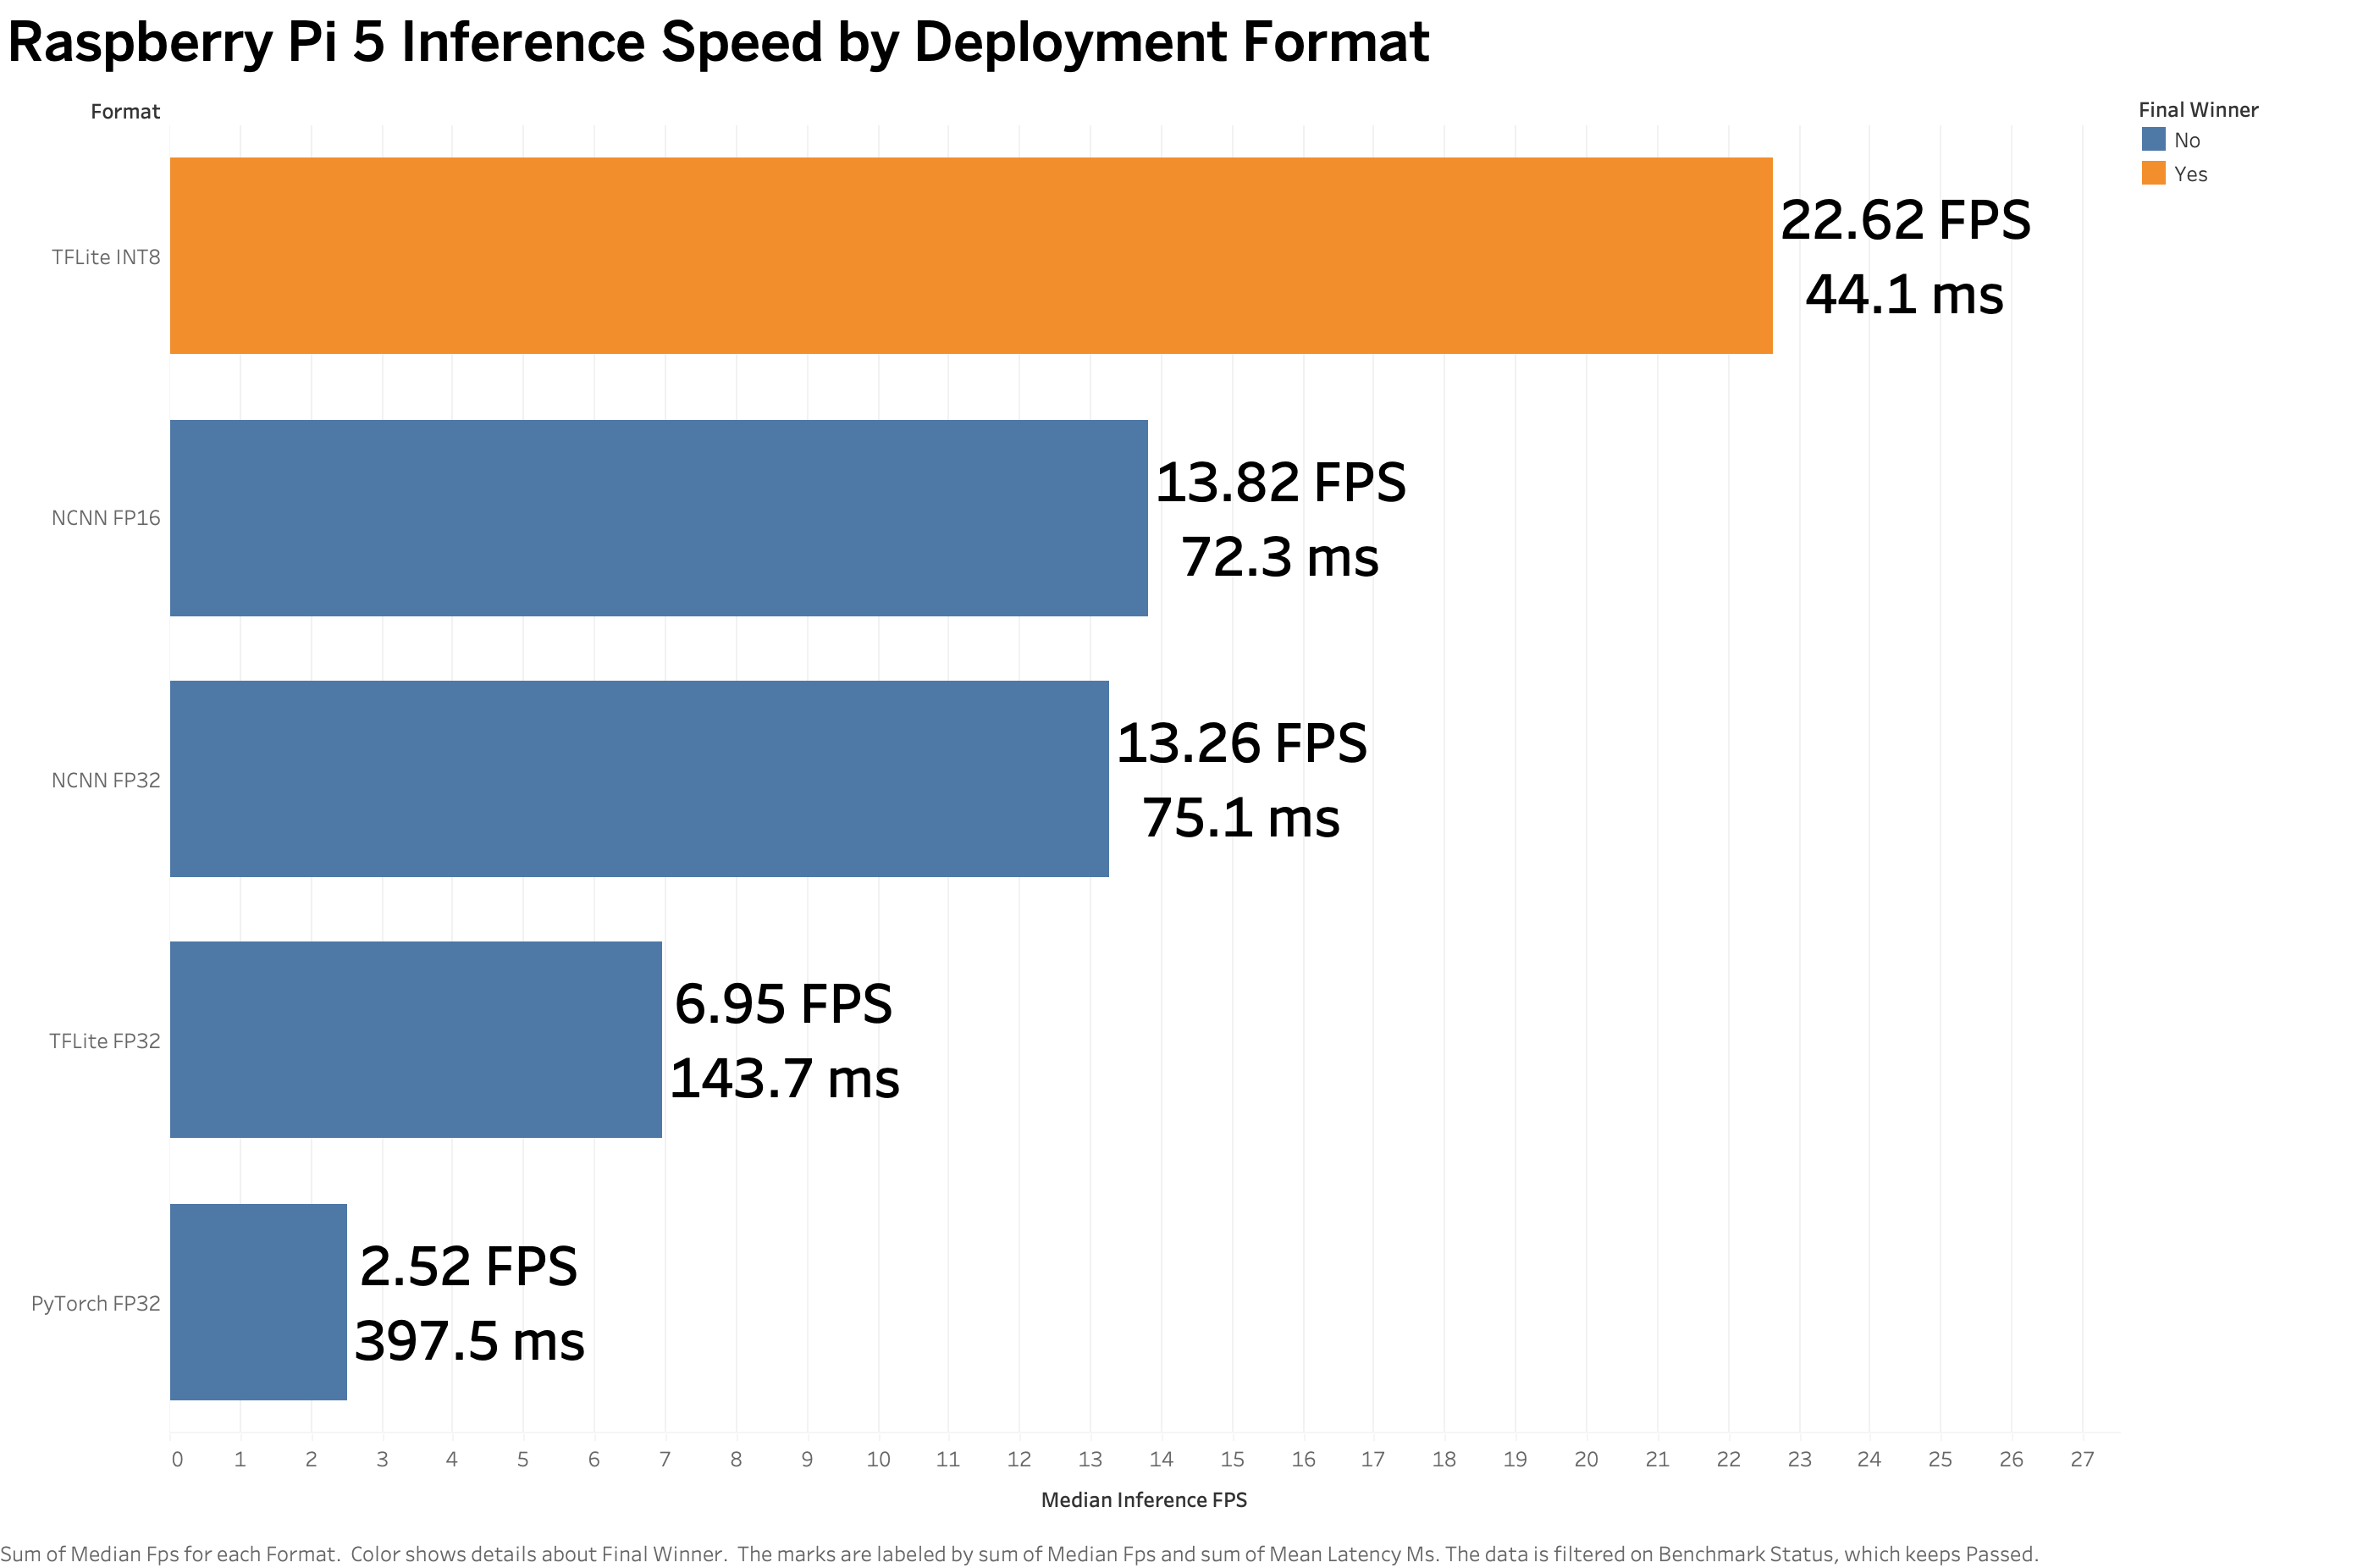
\includegraphics[width=\textwidth,height=4.2cm,keepaspectratio]{figures/figure_09.png}\\[2pt]
    {\tiny Figure 4.3: Median throughput (FPS) and mean latency (ms) across formats on Pi 5.}
  \end{column}
\end{columns}
\end{frame}

% -------------------------------------------------------------
% SLIDE 22: Accuracy vs Throughput Trade-off
% -------------------------------------------------------------
\begin{frame}{Throughput vs Accuracy: A Quantifiable, Acceptable Trade-Off}
\begin{columns}[T]
  \begin{column}{0.48\textwidth}
    \begin{block}{\small Speed vs Accuracy Trade-off}
      \small
      \begin{itemize}
        \item \textbf{PyTorch FP32:} mAP50-95 = 0.275, F1 = 0.622, FPS = 2.52
        \item \textbf{TFLite FP32:} mAP50-95 = 0.270, F1 = 0.599, FPS = 6.95
        \item \textbf{NCNN FP16:} mAP50-95 = 0.270, F1 = 0.600, FPS = 13.82
        \item \textbf{TFLite INT8:} mAP50-95 = 0.234, F1 = 0.594, \textbf{FPS = 22.62}
        \item \textbf{Trade-off Assessment:} A 14.9\% drop in mAP50--95 buys an \textbf{800\% gain in throughput} (2.5 $\rightarrow$ 22.6 FPS). Highly favorable for field deployment.
      \end{itemize}
    \end{block}
  \end{column}
  \begin{column}{0.48\textwidth}
    \centering
    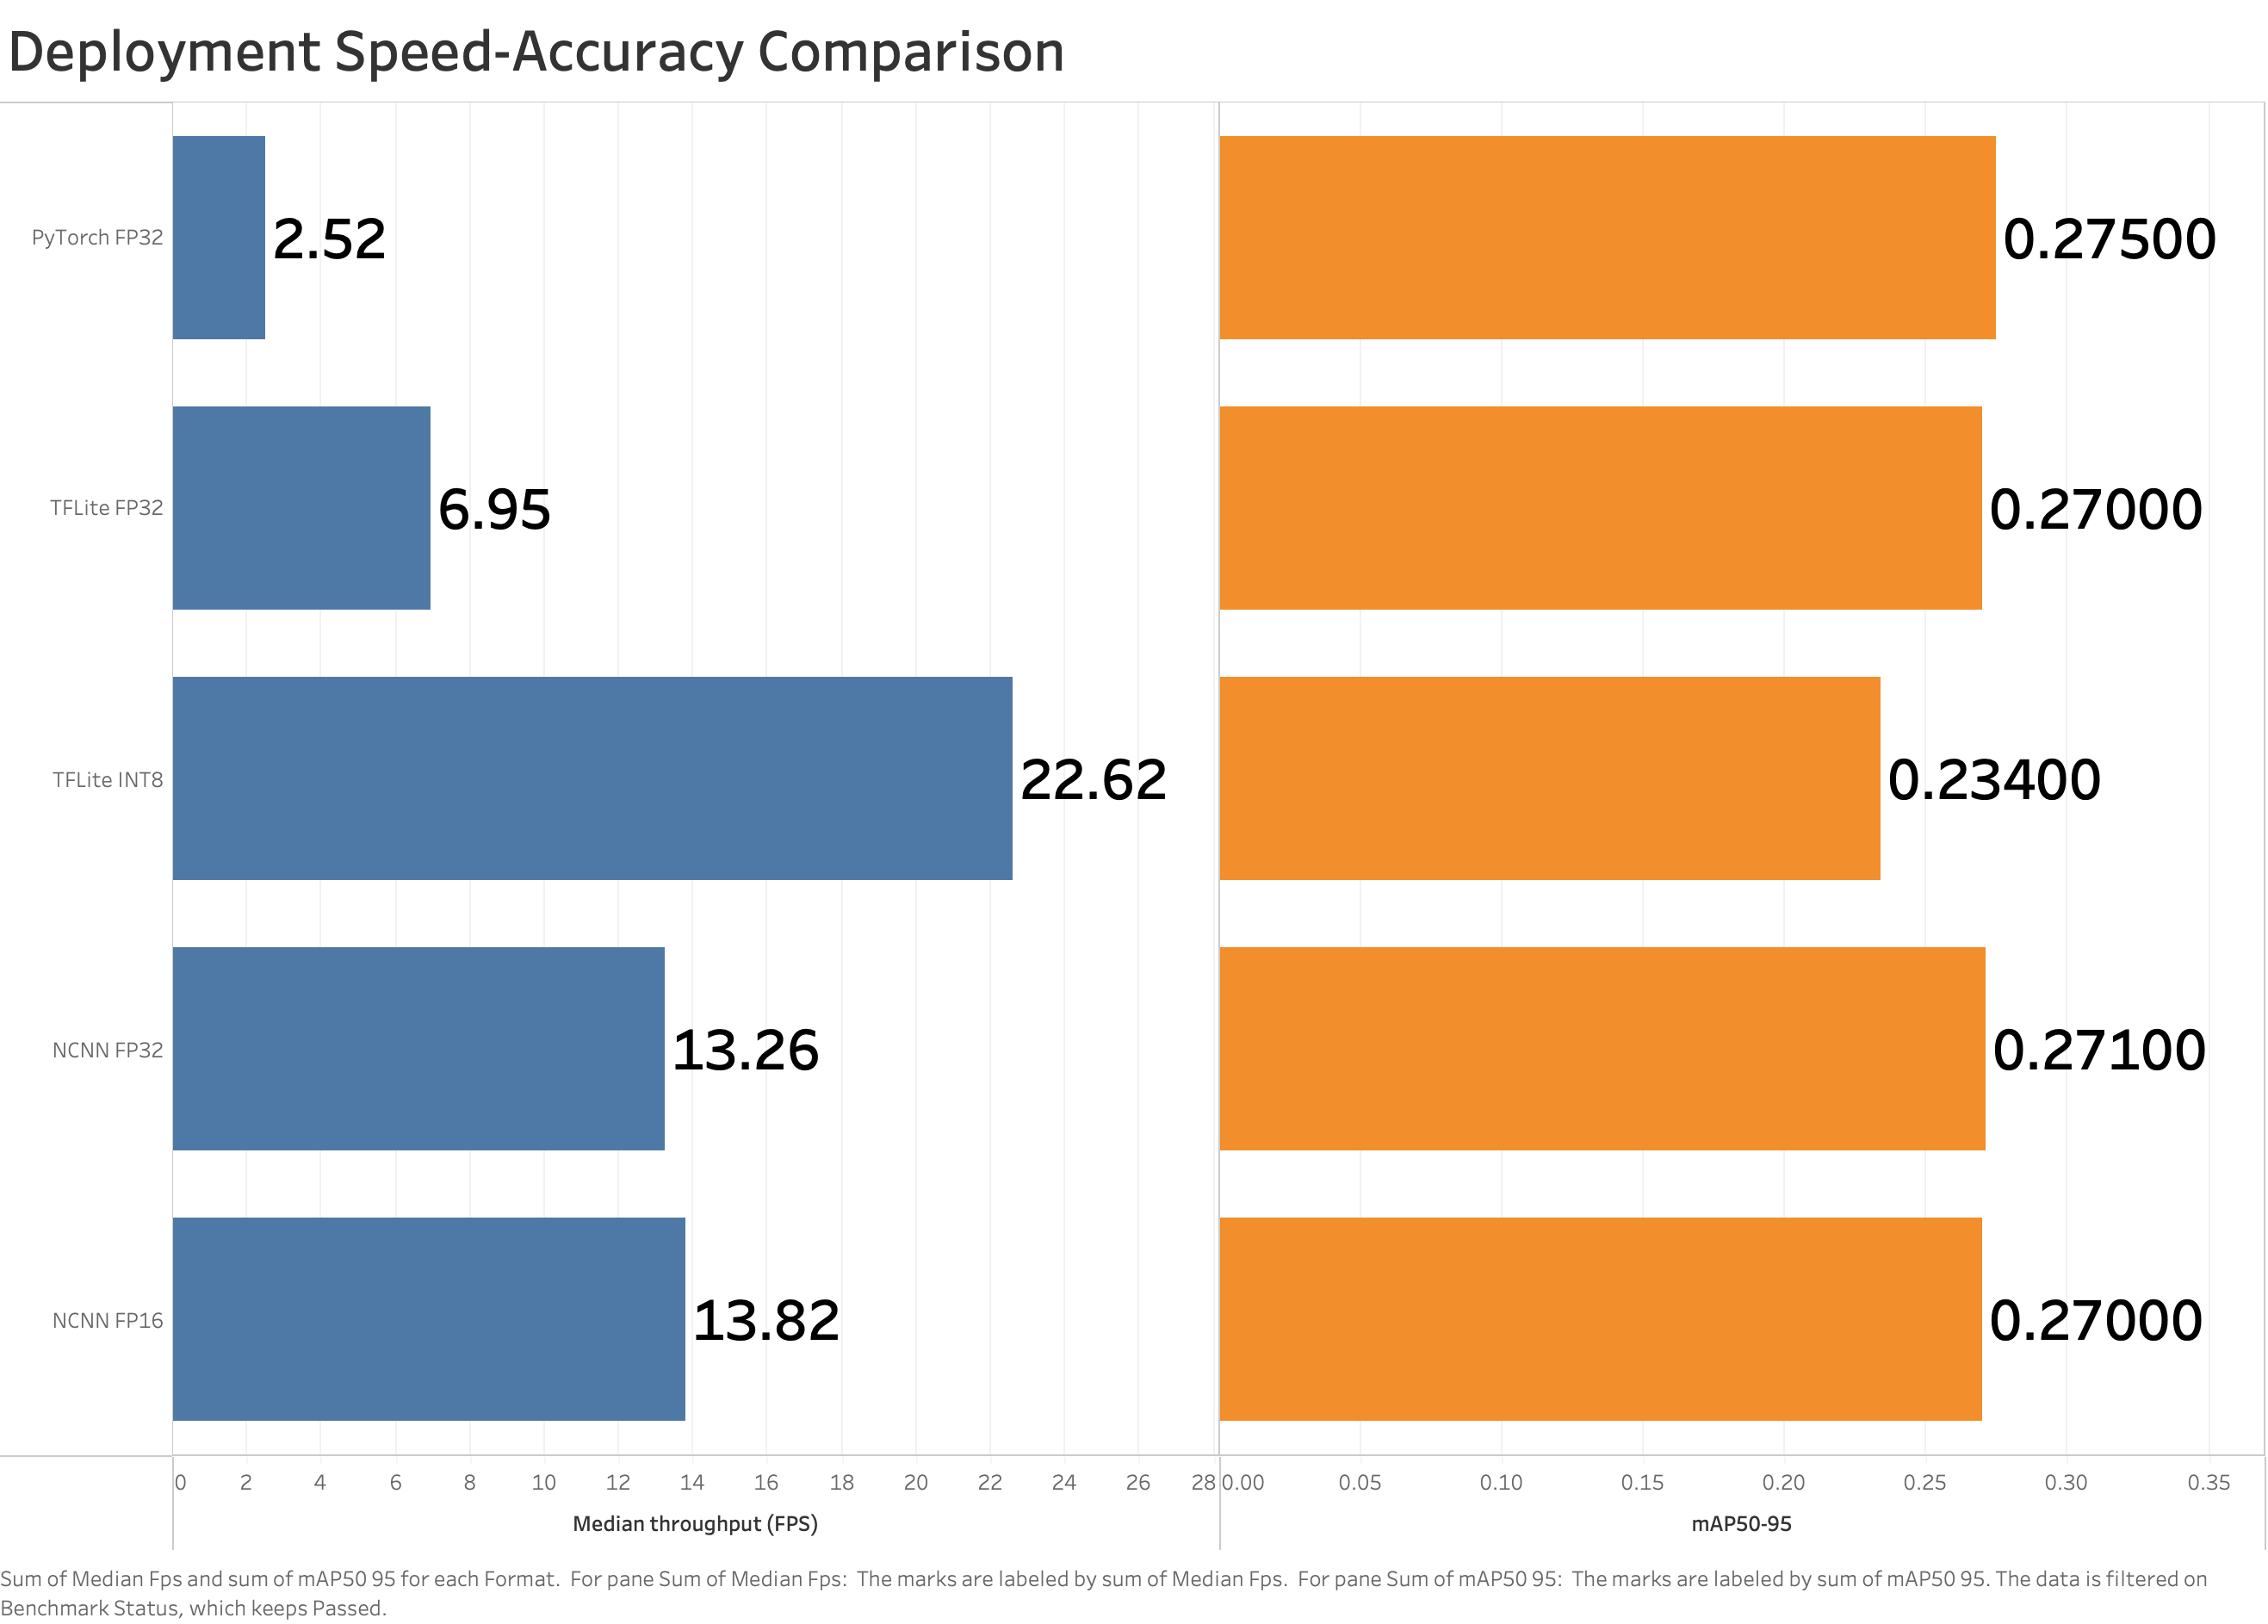
\includegraphics[width=\textwidth,height=4.2cm,keepaspectratio]{figures/figure_deployment_speed_accuracy_scatter.png}\\[2pt]
    {\tiny Figure 4.2: Median throughput vs mAP50--95 Pareto scatter plot.}
  \end{column}
\end{columns}
\end{frame}

% -------------------------------------------------------------
% SLIDE 23: Resource & Thermal Diagnostics
% -------------------------------------------------------------
\begin{frame}{System Resources: INT8 Optimises CPU, Memory \& Thermal Load}
\begin{columns}[T]
  \begin{column}{0.48\textwidth}
    \begin{block}{\small Hardware Utilisation on Raspberry Pi 5}
      \small
      \begin{itemize}
        \item \textbf{Peak Process Memory:} TFLite INT8 used the least RAM: \textbf{824.2 MB} (vs 868.3 MB for TFLite FP32).
        \item \textbf{CPU Core Load:} TFLite INT8 required \textbf{62.8\%} CPU load, leaving headroom for camera capture and telemetry.
        \item \textbf{Thermal Dissipation:} TFLite INT8 ran coolest at \textbf{55.10\,$^\circ$C} (vs 66.10\,$^\circ$C for TFLite FP32).
        \item Integer SIMD instructions generate significantly less thermal dissipation.
      \end{itemize}
    \end{block}
  \end{column}
  \begin{column}{0.48\textwidth}
    \centering
    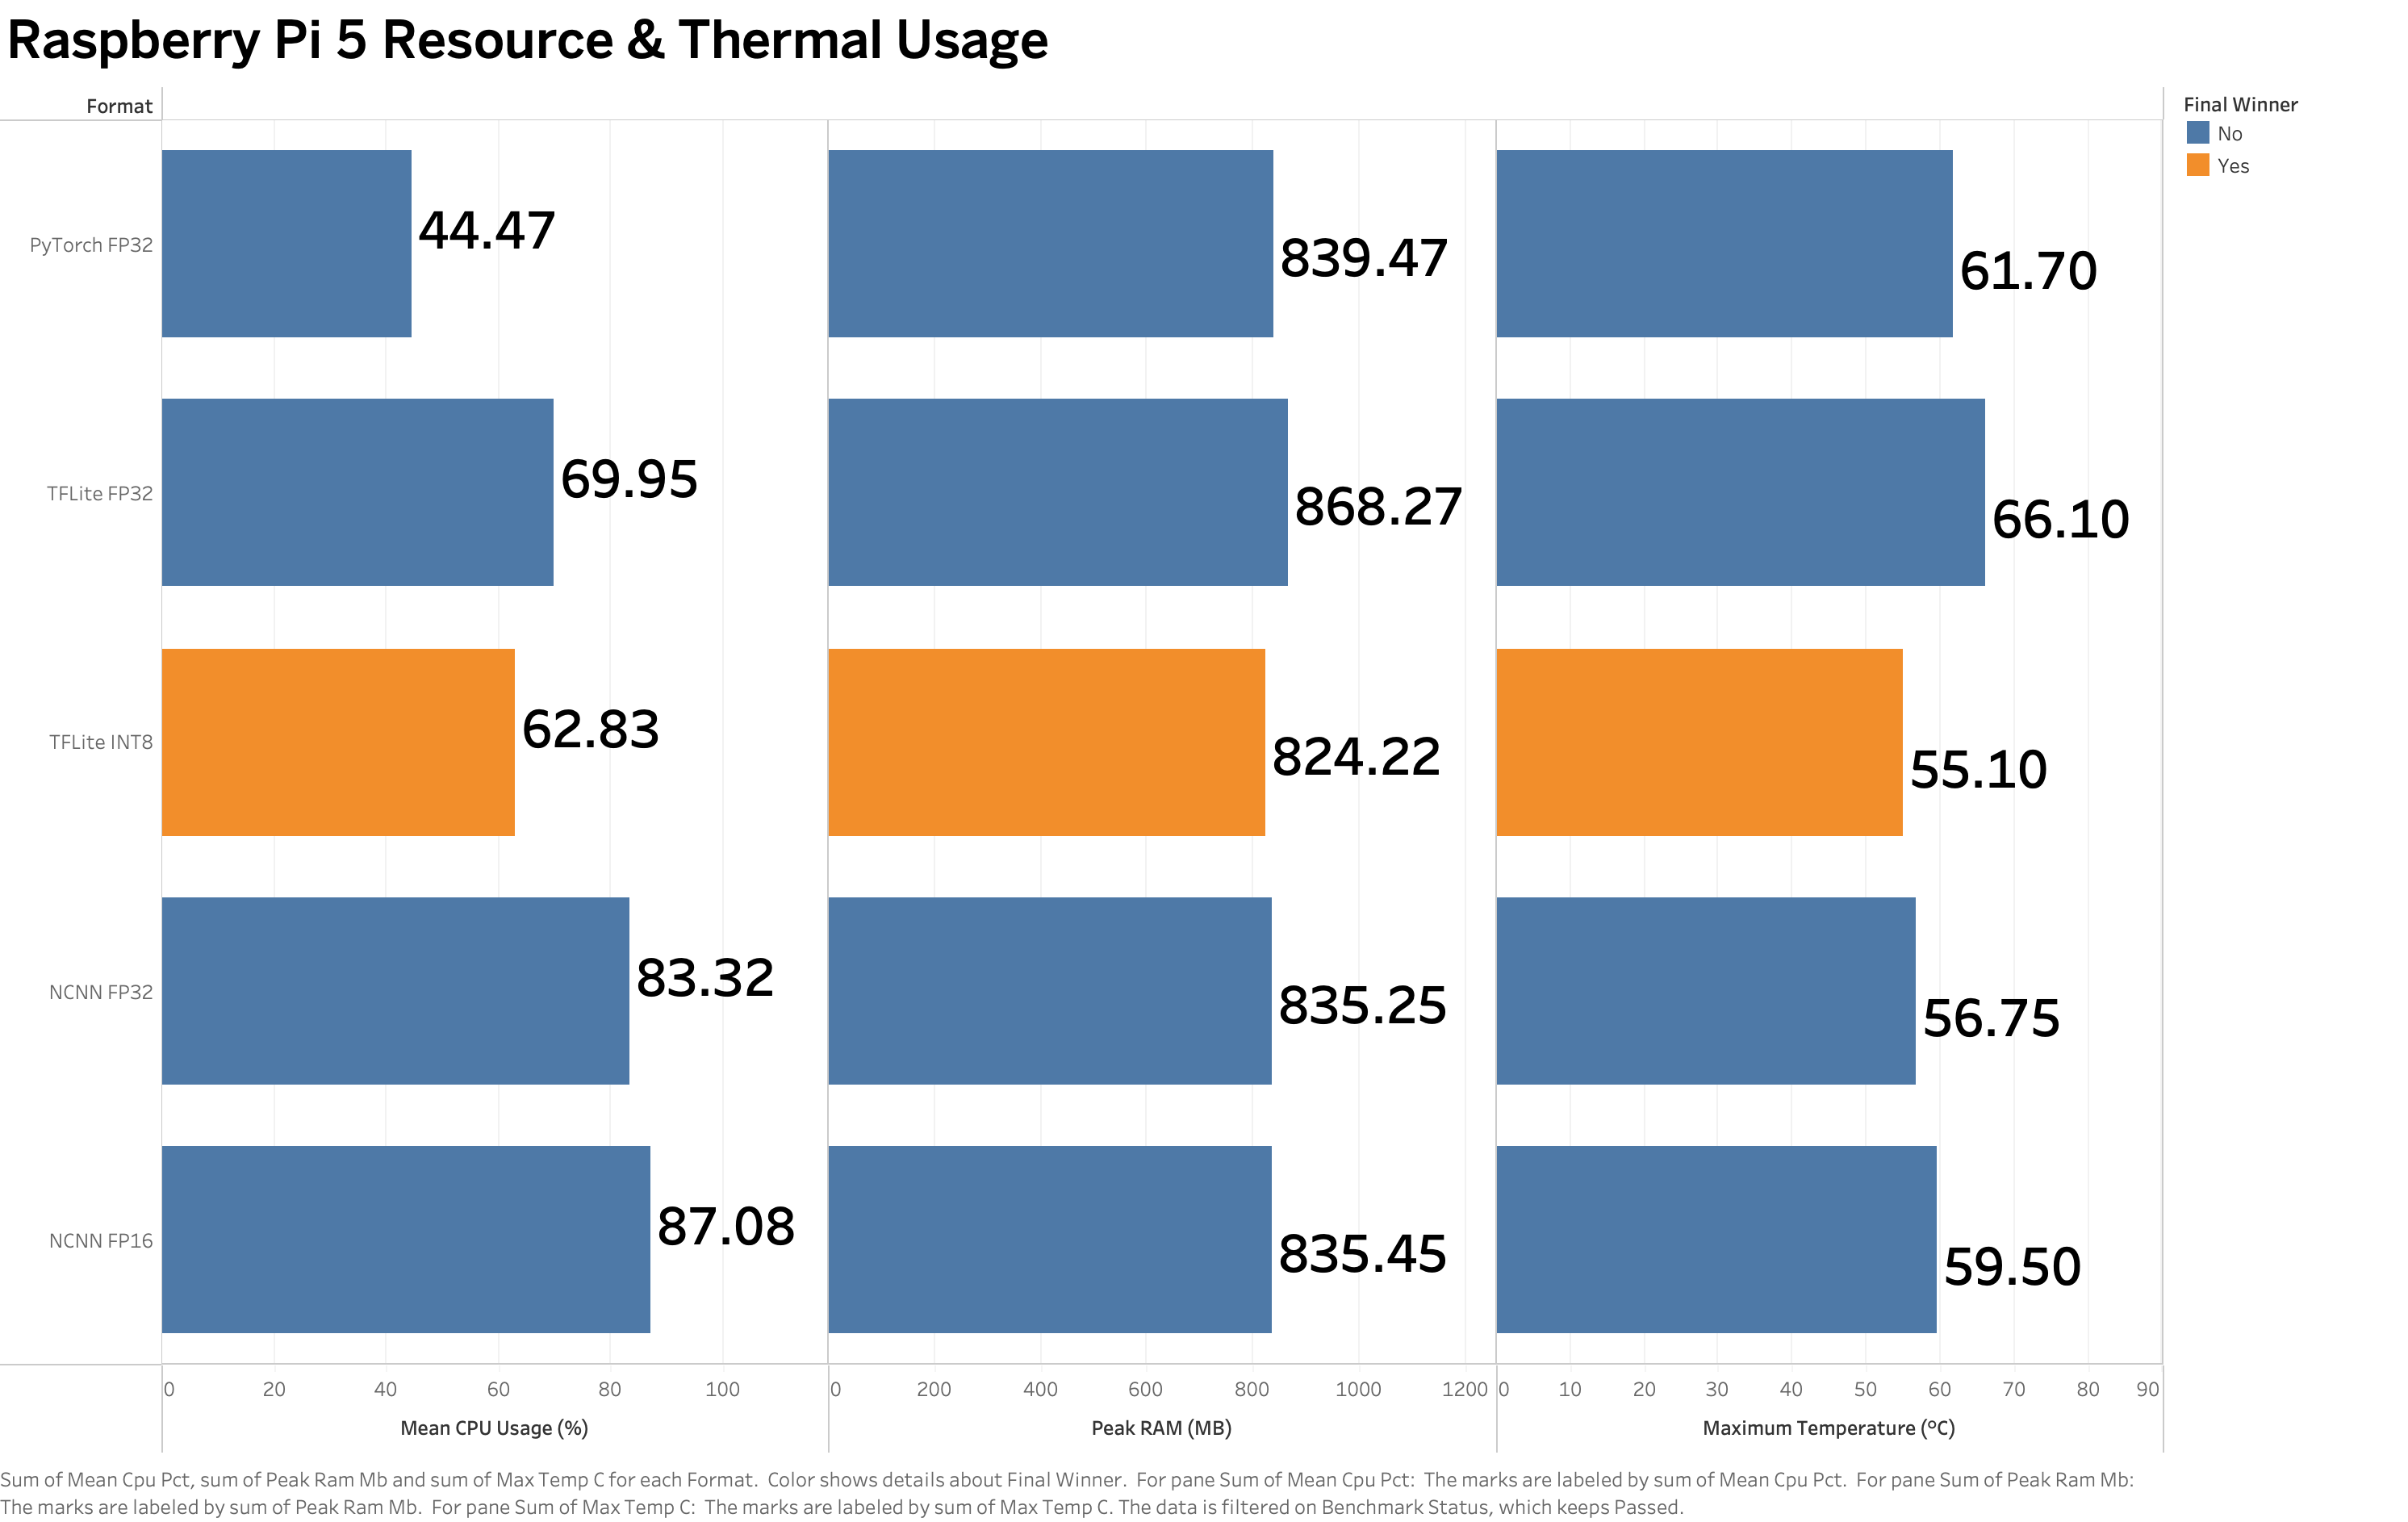
\includegraphics[width=\textwidth,height=4.2cm,keepaspectratio]{figures/figure_11.png}\\[2pt]
    {\tiny Figure 4.5: CPU load, peak RAM, and short-run temperature across formats.}
  \end{column}
\end{columns}
\end{frame}

% -------------------------------------------------------------
% SLIDE 24: Operational Stability
% -------------------------------------------------------------
\section{Operational Stability}
\begin{frame}{Stability Testing Exposes Critical Runtime Failures}
\begin{columns}[T]
  \begin{column}{0.48\textwidth}
    \begin{block}{\small Negative Results \& Runtime Crashes}
      \small
      \begin{itemize}
        \item \textbf{Export success does not guarantee edge stability!}
        \item \textbf{ONNX FP32 Fatal Failure:} Exported cleanly, but crashed completely during benchmark aggregation on ARM64.
        \item \textbf{NCNN Endurance Crash:} Passed 90-image benchmark, but crashed during continuous 10-pass endurance run due to thread contention.
      \end{itemize}
    \end{block}
  \end{column}
  \begin{column}{0.48\textwidth}
    \begin{block}{\small Robustness \& Deployment Findings}
      \small
      \begin{itemize}
        \item \textbf{TFLite INT8 Winner:} The \textbf{only} format that completed 100\% of both fixed benchmark and continuous endurance runs without failure.
        \item \textbf{System-Level Validation:} Highlights the critical necessity of measuring on target physical hardware under real workload stress.
        \item \textbf{Reporting Integrity:} Disclosing runtime failures prevents flawed assumptions about portable model equivalence.
      \end{itemize}
    \end{block}
  \end{column}
\end{columns}
\end{frame}

% -------------------------------------------------------------
% SLIDE 25: Final Decision & Roadmap
% -------------------------------------------------------------
\section{Conclusions \& Roadmap}
\begin{frame}{Final Selection: TFLite INT8 Validated; Future Roadmap Defined}
\begin{columns}[T]
  \begin{column}{0.48\textwidth}
    \begin{block}{\small Final Selection: TFLite INT8}
      \small
      \begin{itemize}
        \item \textbf{Speed:} 22.62 FPS ($9.01\times$ speedup, $>20$ FPS threshold).
        \item \textbf{Localisation:} Retains 0.234 mAP50--95, 0.633 count MAE.
        \item \textbf{Efficiency:} Lowest RAM (824 MB) and lowest temperature (55.1\,$^\circ$C).
        \item \textbf{Reliability:} 100\% stability across all continuous runs.
        \item \textbf{Hypotheses Supported:} H1 (Speedup), H2 (Accuracy Cost), and H3 (Stability Divergence) fully validated.
      \end{itemize}
    \end{block}
  \end{column}
  \begin{column}{0.48\textwidth}
    \begin{block}{\small Prioritised Future Roadmap}
      \small
      \begin{enumerate}
        \item \textbf{3D Depth Sensing:} Integrate stereo vision / LiDAR to elevate half-buried detection above 35\%.
        \item \textbf{Live Video Stream:} Build GStreamer pipeline with GPS geo-tagging.
        \item \textbf{NPU Acceleration:} Deploy on Raspberry Pi AI Kit (Hailo-8L NPU, 13 TOPS) for $<10$~ms latency.
        \item \textbf{Actuator Integration:} Connect to hydraulic rock picker PLC via CAN bus.
      \end{enumerate}
    \end{block}
  \end{column}
\end{columns}
\end{frame}

\end{document}
